
\chapter{绪论}\label{chap:introduction}

Several engineering applications where the Navier-Stokes-Fourier equations fail to predict the behavior of rarefied gas flows are introduced, as well as the simple gas kinetic theory and molecular dynamics simulation.


\section{气体的性质}


一定宏观体积的气体由大量分子组成,这些分子以相当不规则的方式不断地运动。其运动状态的改变由分子间的相互作用力决定。一般用Lennard-Jones势描述分子间相互作用
\begin{equation}\label{Lennard_Jones_chapter}
\phi(r)=4\epsilon\left[\left(\frac{d_{LJ}}{r}\right)^{12}-\left(\frac{d_{LJ}}{r}\right)^6\right],
\end{equation}
where $\epsilon$ is the potential depth and $d_{LJ}$ is the distance at which the potential between two molecules is zero.

这种巨大的自由度使得每个分子的轨迹变得不可能。



\subsection{气体分子间的相互作用}

\subsection{理想气体}

\subsection{压强、温度、内能}

\subsection{平均自由程}

\subsection{简单输运现象}

\newpage

\section{Navier-Stokes-Fourier equations}

%\index{Navier-Stokes-Fourier equations}
\index{density}
\index{velocity}
\index{temperature}
\index{pressure}
\index{heat flux}
\index{conservation}
\index{acceleration}
\index{internal energy}
%\index{spatial coordinate}



The fundamental and practical task in the study of gas dynamics is to obtain the macroscopic quantities, such as the mass density $\rho$, bulk velocity $\bm{u}$, temperature $T$, pressure tensor
%\footnote{Note that while the stress $\bm{\tau}$ in continuum mechanics is understood to be the force per unit area that the part lying on the positive side of a surface element exerts on the part lying on the negative side, the pressure tensor $\bm{p}$ in this book has an opposite sign: $\bm{p}=-\bm{\tau}$.} 
$\bm{p}$, and heat flux $\bm{q}$. Traditionally, the gas is treated as a continuum and the following equations are built based on the mass, momentum, and energy conservation:
\begin{equation}\label{macro}
\begin{aligned}[b]
\frac{\partial \rho}{\partial t}+\frac{\partial(\rho{}u_j) }{\partial x_j}=0, \\
\frac{\partial (\rho{u_i})}{\partial t}+\frac{\partial (\rho{}u_iu_j+p_{ij})}{\partial x_j}= \rho{}a_i,\\
\frac{\partial \left(\rho{}E\right)}{\partial t}+\frac{\partial \left(\rho{}{E}u_j+u_i{p}_{ij}+q_j\right)}{\partial x_j}=\rho{}a_ju_j,
\end{aligned}
\end{equation} 
where $t$ is the time, $\bm{x}\equiv(x_1,x_2,x_3)$ is the spatial Cartesian coordinates, $\bm{a}\equiv(a_1,a_2,a_3)$ is the external acceleration, and $E\equiv{}e+u_iu_i/{2}$ is the specific energy with $e$ being the specific internal energy that is a function of temperature $T$. The subscripts $i,j,k=1,2,3$ represent the three orthogonal spatial directions, and the Einstein summation convention is used. 

% ; for single-species gases, 
%\begin{equation}
%e=\frac{3+d_i}{2}\frac{k_B}{m}T,
%\end{equation}
%where $k_B$ is the Boltzmann constant, $m$ is the molecular mass, and $d_i$ is the internal degrees of freedom

Equation~\eqref{macro} is not closed because expressions for the pressure tensor $\bm{p}$ and heat flux $\bm{q}$ can not be determined from conservation laws. Usually, the phenomenological and empirical constitutive relations \index{constitutive relation} are adopted, e.g., Newton's law of viscosity \index{Newton's law of stress}
\begin{equation}\label{shear_Chapter1_stress}
\begin{aligned}[b]
p_{ij}=\frac{\rho{}k_BT}{m}\delta_{ij}-
\mu\left(\frac{\partial u_i}{\partial x_j}+\frac{\partial u_j}{\partial x_i}
-\frac{2}{3}\frac{\partial u_k}{\partial x_k}\delta_{ij}\right)
-\mu_b\frac{\partial u_k}{\partial x_k}\delta_{ij},
\end{aligned}
\end{equation}
and Fourier's law of heat conduction \index{Fourier's law of heat conduction}
\begin{equation}\label{heat_Chapter1_conduction}
\begin{aligned}[b]
q_i=-\kappa\frac{\partial T}{\partial x_i},
\end{aligned}
\end{equation}
where $k_B$ is the Boltzmann constant, $m$ is the molecular mass, $\delta$ is the Kronecker delta, $\mu$ is the shear viscosity, $\mu_b$ is the bulk viscosity, and $\kappa$ is the thermal conductivity. 

\index{molecular mass}
\index{bulk viscosity}
\index{shear viscosity}
\index{thermal conductivity}
\index{Kronecker delta}
\index{Chapman-Enskog expansion!Navier-Stokes-Fourier}

Together with the non-velocity-slip and non-temperature-jump conditions at the solid surface, the Navier-Stokes-Fourier (NSF) equations have found a wide range of engineering applications. 


\section{Continuum breakdown}\label{continuum_breakdown}

However, in some extreme conditions, the gas dynamics predicted by NSF equations can differ from experimental results significantly. The gas flow where the traditional NSF equations fail is called rarefied gas flow, and its dynamics is rarefied gas dynamics (RGD). It is also called non-equilibrium gas dynamics because, as we shall see in later chapters, the velocity distribution function of gas molecules departures from the Maxwell equilibrium distribution significantly. Sometimes it is also called non-continuum gas dynamics. This is because the basic assumption in continuum mechanics that ``the stress at a point is related to the strain and the rate of change of strain with respect to time at the same point'' is violated.  

Typical examples of rarefaction effects that lead to non-intuitive phenomena beyond the description of NSF equations, with applications from the sky, earth surface, and underground, are briefly illustrated below.  

\subsection{Reentry of space vehicle}

%Atmospheric entry is the movement of an object from outer space into and through the gases of earth's atmosphere, including the uncontrolled entry, such as the entry of astronomical objects, space debris, or bolides, and the controlled entry of a spacecraft capable of being navigated or following a predetermined course. 

\begin{figure}[t]
	\centering
	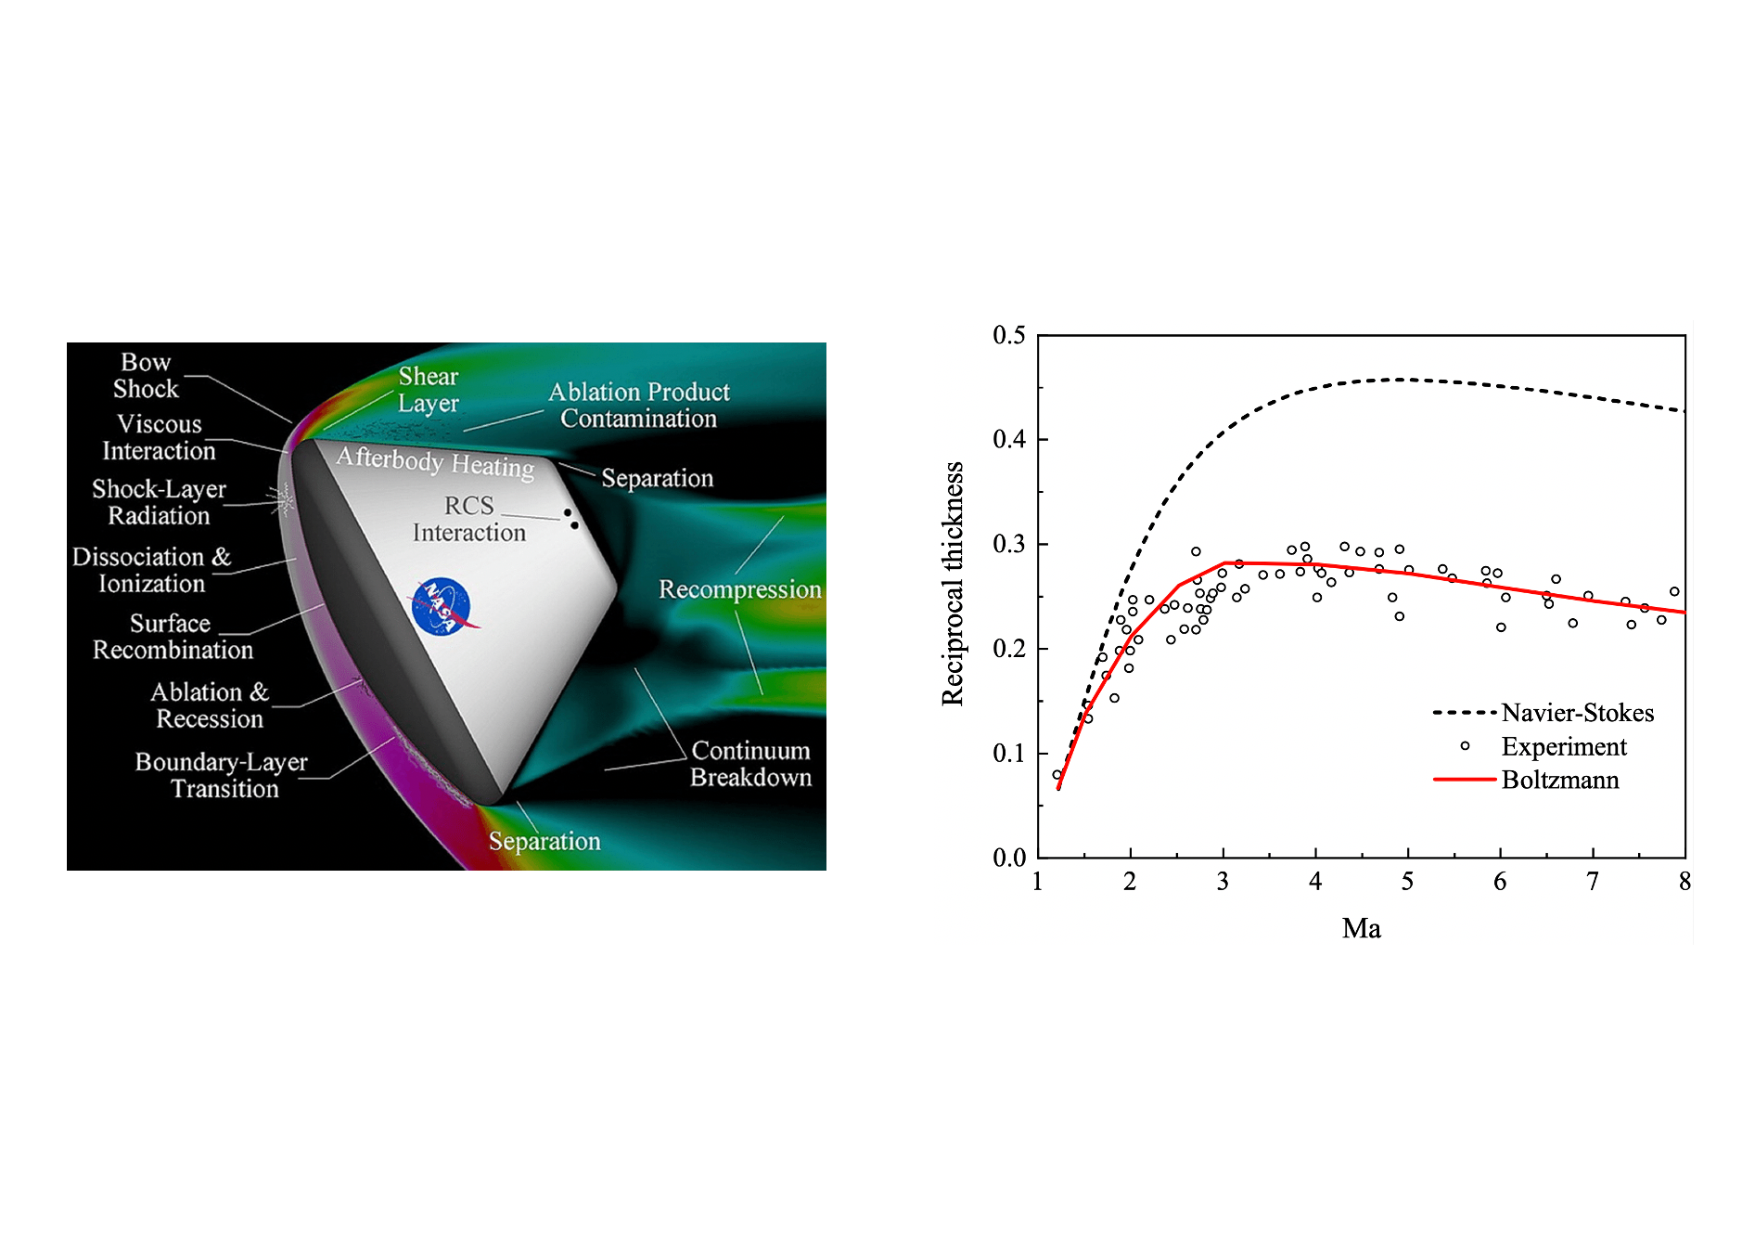
\includegraphics[scale=0.5]{Introduction/IMG/Re_entry.pdf}
	\vskip 0.5cm
	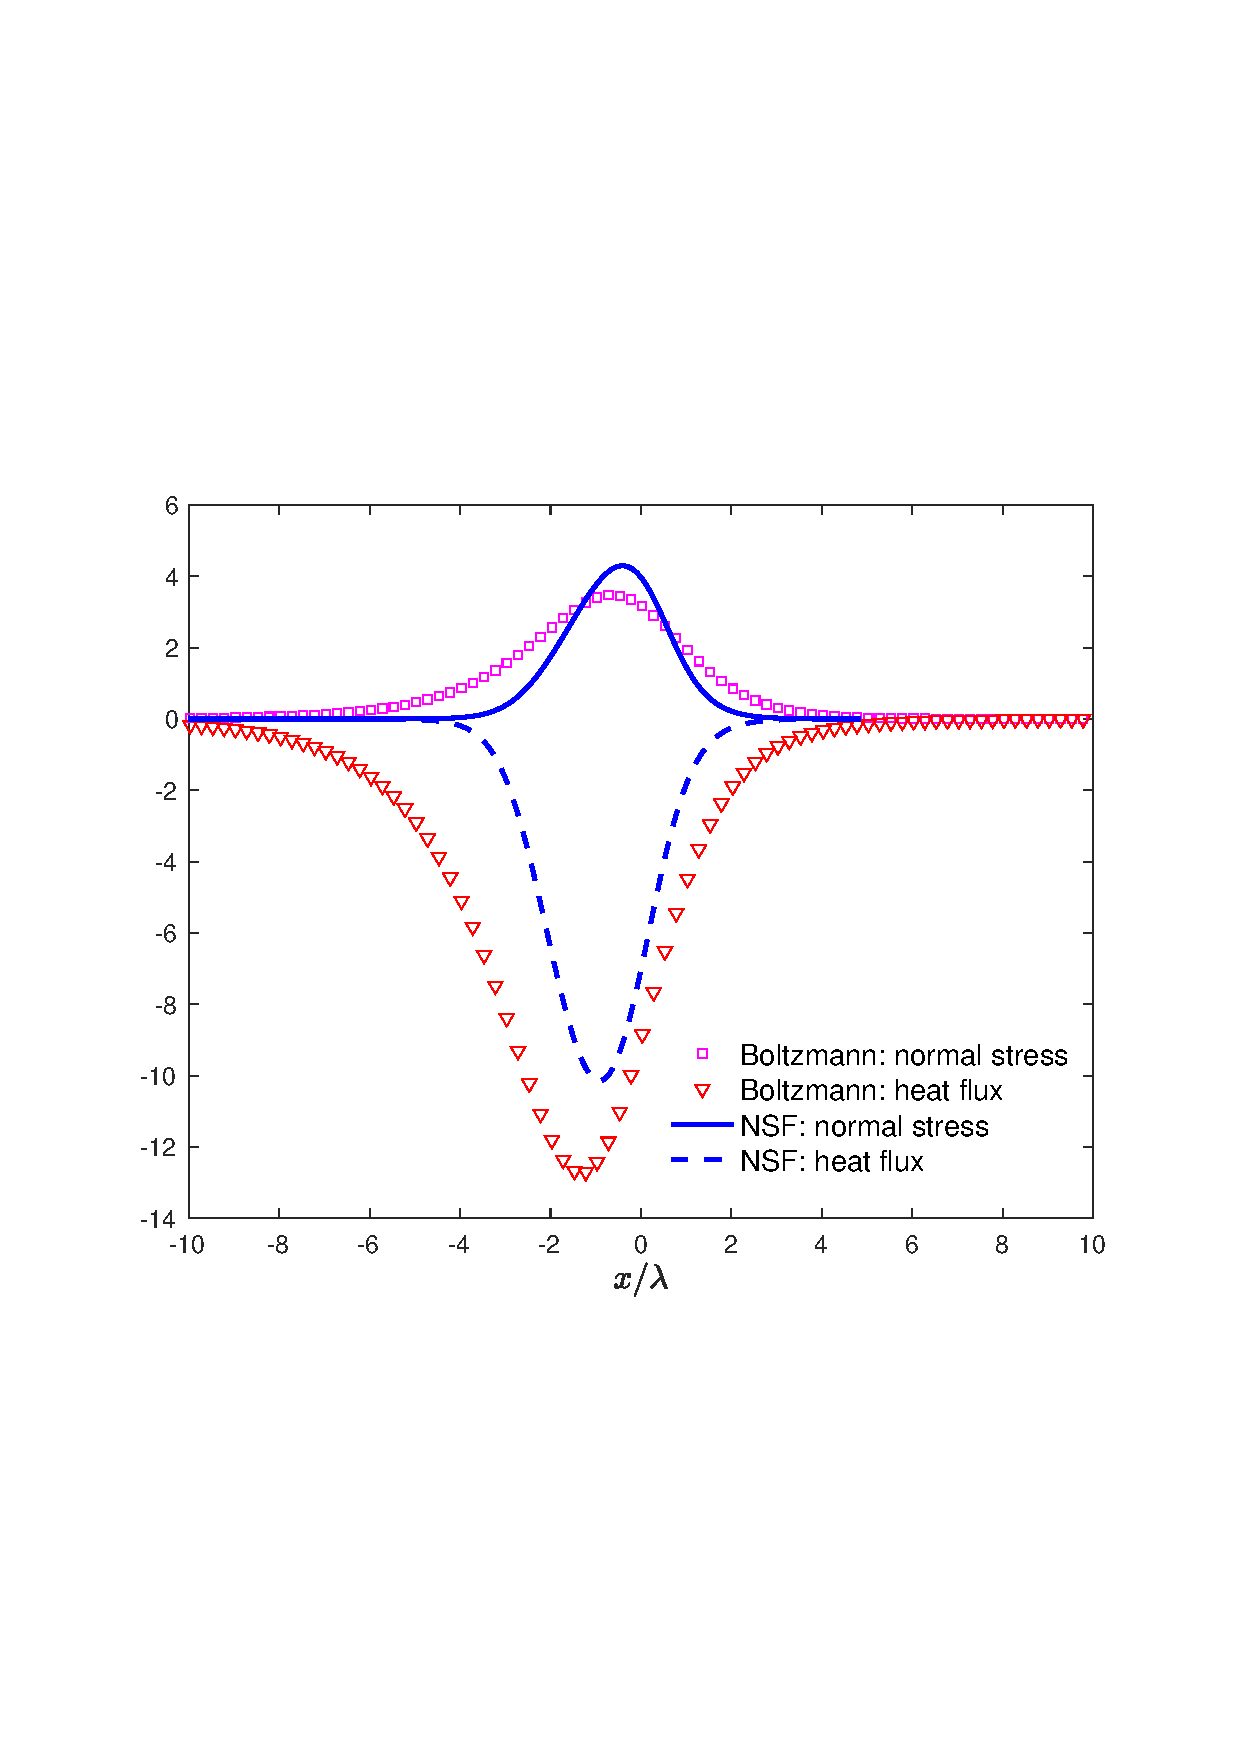
\includegraphics[scale=0.4]{Introduction/IMG/Boltzmann_NS_shockMa4.pdf}
	\caption{
		(Left) Complicated gas dynamics around the reentry capsule (image credit: NASA). (Right) Inverse thickness of the normal shock wave of argon as a function of the Mach number~\cite{Alsmeyer1976JFM}. (Bottom) Dimensionless normal stress and heat flux of argon shock wave with a Mach number of 4; the distance is normalized by the mean free path $(\lambda)$ of the gas in upstream. 
		%Validation of the Boltzmann equation will be given in Chapter~\ref{chap:single_component}.
	}
	\label{Re_entry}
\end{figure}

% where the space vehicle moves with a velocity of about 7.8 km/s when returning from the International Space Station

Figure~\ref{Re_entry} sketches the complex flow physics around a reentry vehicle, where the reentry speed is about 8 km/s. Due to the violent interaction with atmosphere, a strong bow shock wave is generated in front of the vehicle. Intermolecular collisions also promote energy exchanges among the translational and internal (rotational, vibrational and electronic) modes, and eventually leads to non-equilibrium chemical reactions. Behind the shock wave, a massive amount of the kinetic energy of free stream is converted into the internal energy of surrounding gas, resulting in intense convective and radiative heating to the space vehicle. Meanwhile, supersonic expansion, flow separation, re-circulation, and re-compression take place as the flow passes through the vehicle.


Even for the simple normal shock wave, the NSF equations fail to predict its thickness when the Mach number is larger than 2. Although the thickness of shock wave is only a few mean free path (MFP, the average distance traveled by a moving molecule) of gas molecules, in high altitude flight it is comparable to the dimension of space vehicle and hence the rarefaction effects are significant. On the contrary, the Boltzmann equation well predicts the thickness of normal shock wave over a wide range of Mach number. When the Mach number is 4, the normal stress and heat flux predicted from NSF equations are quite different from those of the Boltzmann equation, which further confirms the failure of NSF equations. In-depth knowledge of RGD is key to predicting/controlling the entry of space objects.

\index{shock wave}
\index{Mach number}
\index{mean free path}


\subsection{Microelectromechanical systems}

\begin{figure}[t]
	\centering
	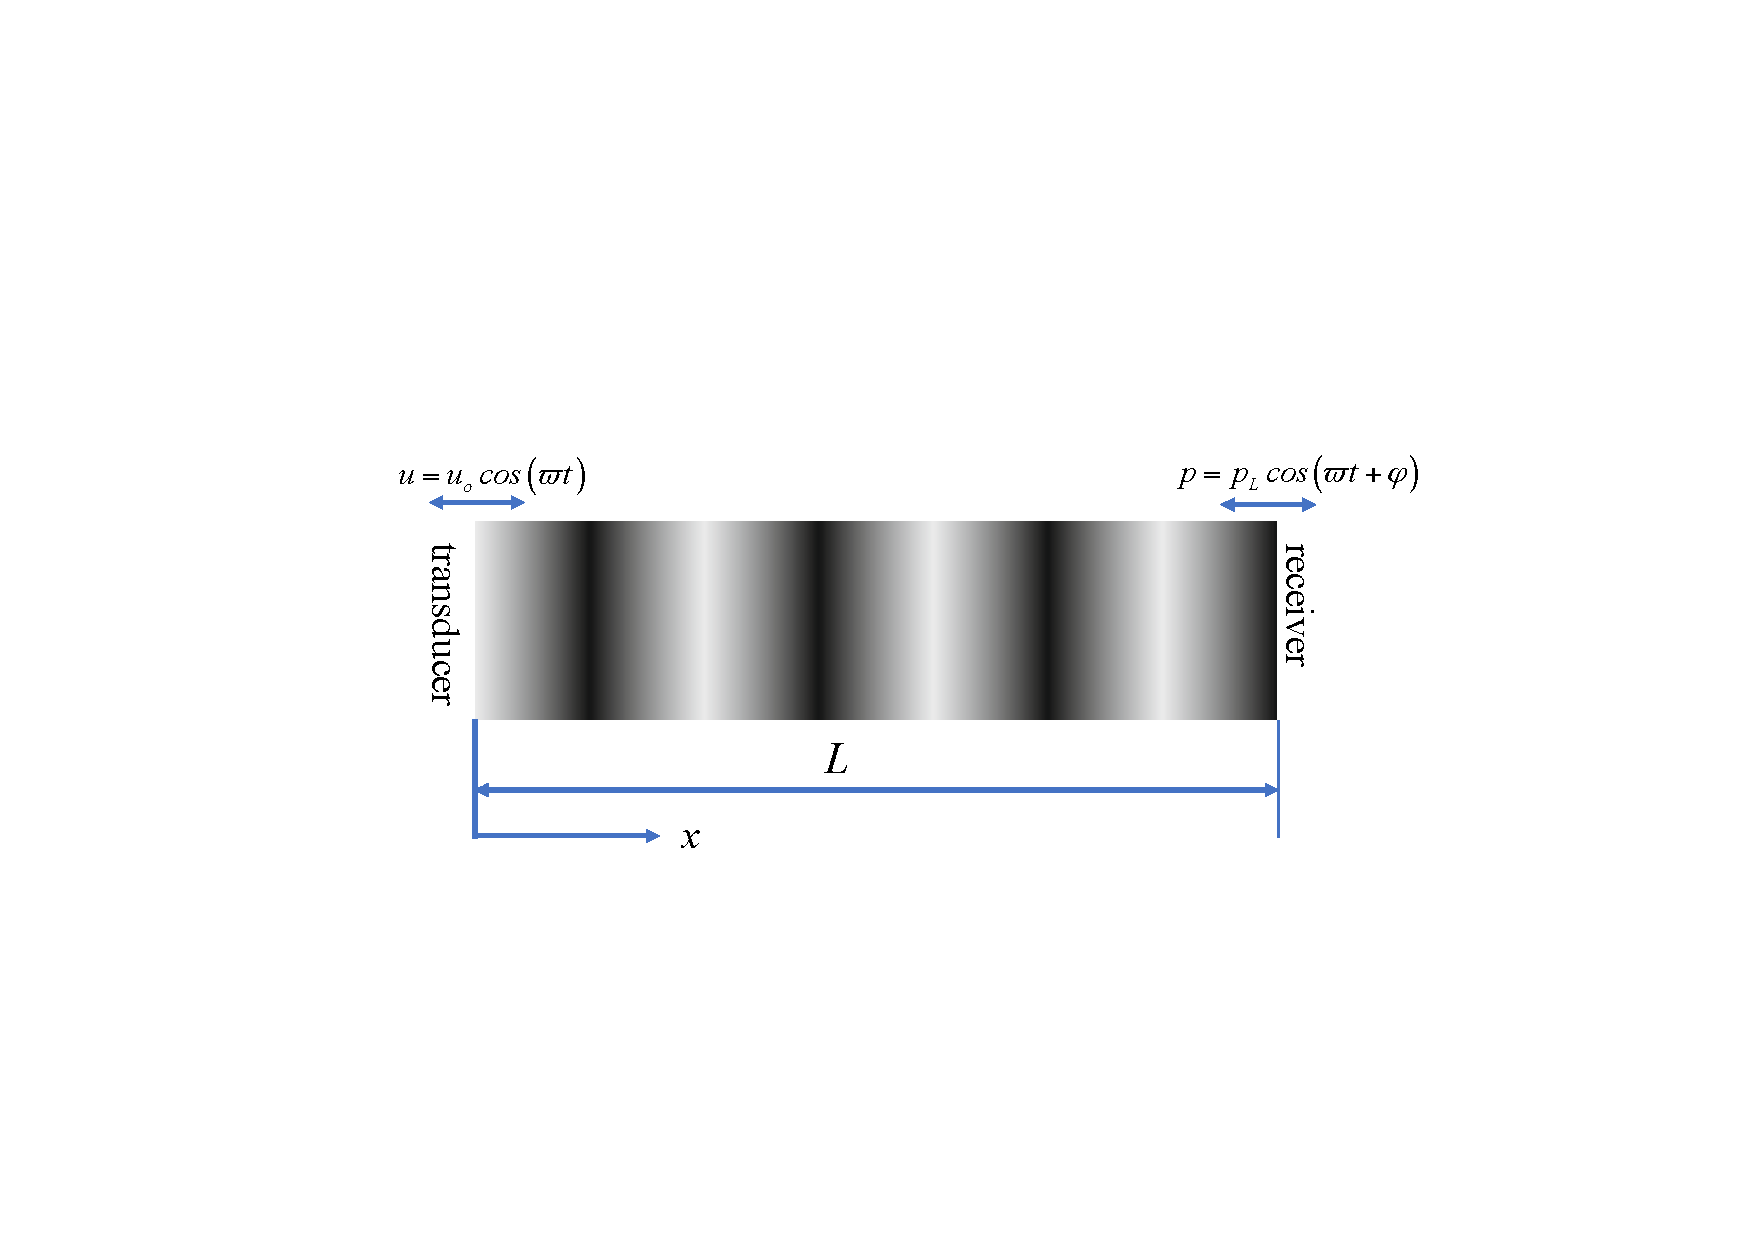
\includegraphics[scale=0.45,viewport=20 10 540 200,clip=true]{Introduction/IMG/resonance.pdf}
	\vskip 0.5cm
	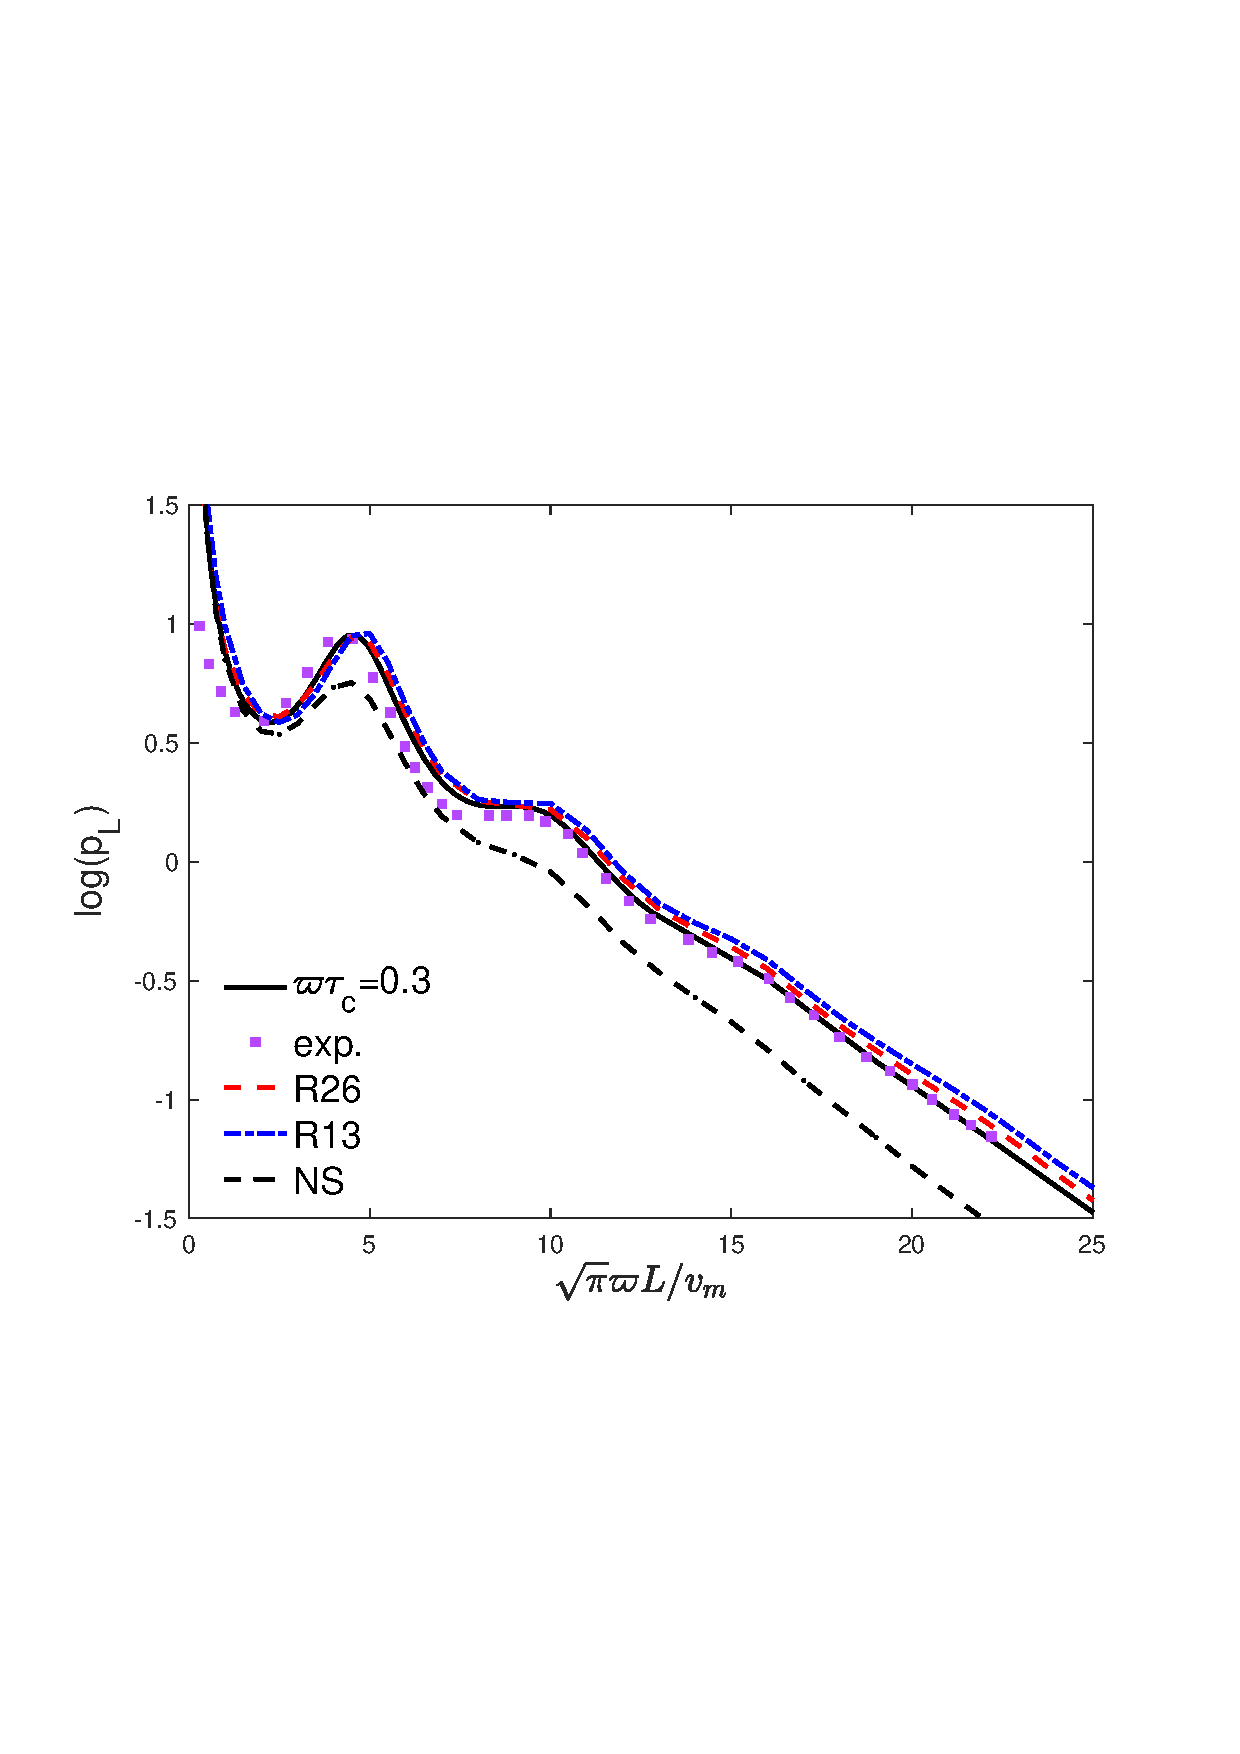
\includegraphics[width=0.45\textwidth]{Introduction/IMG/testOmgTau03.pdf}
	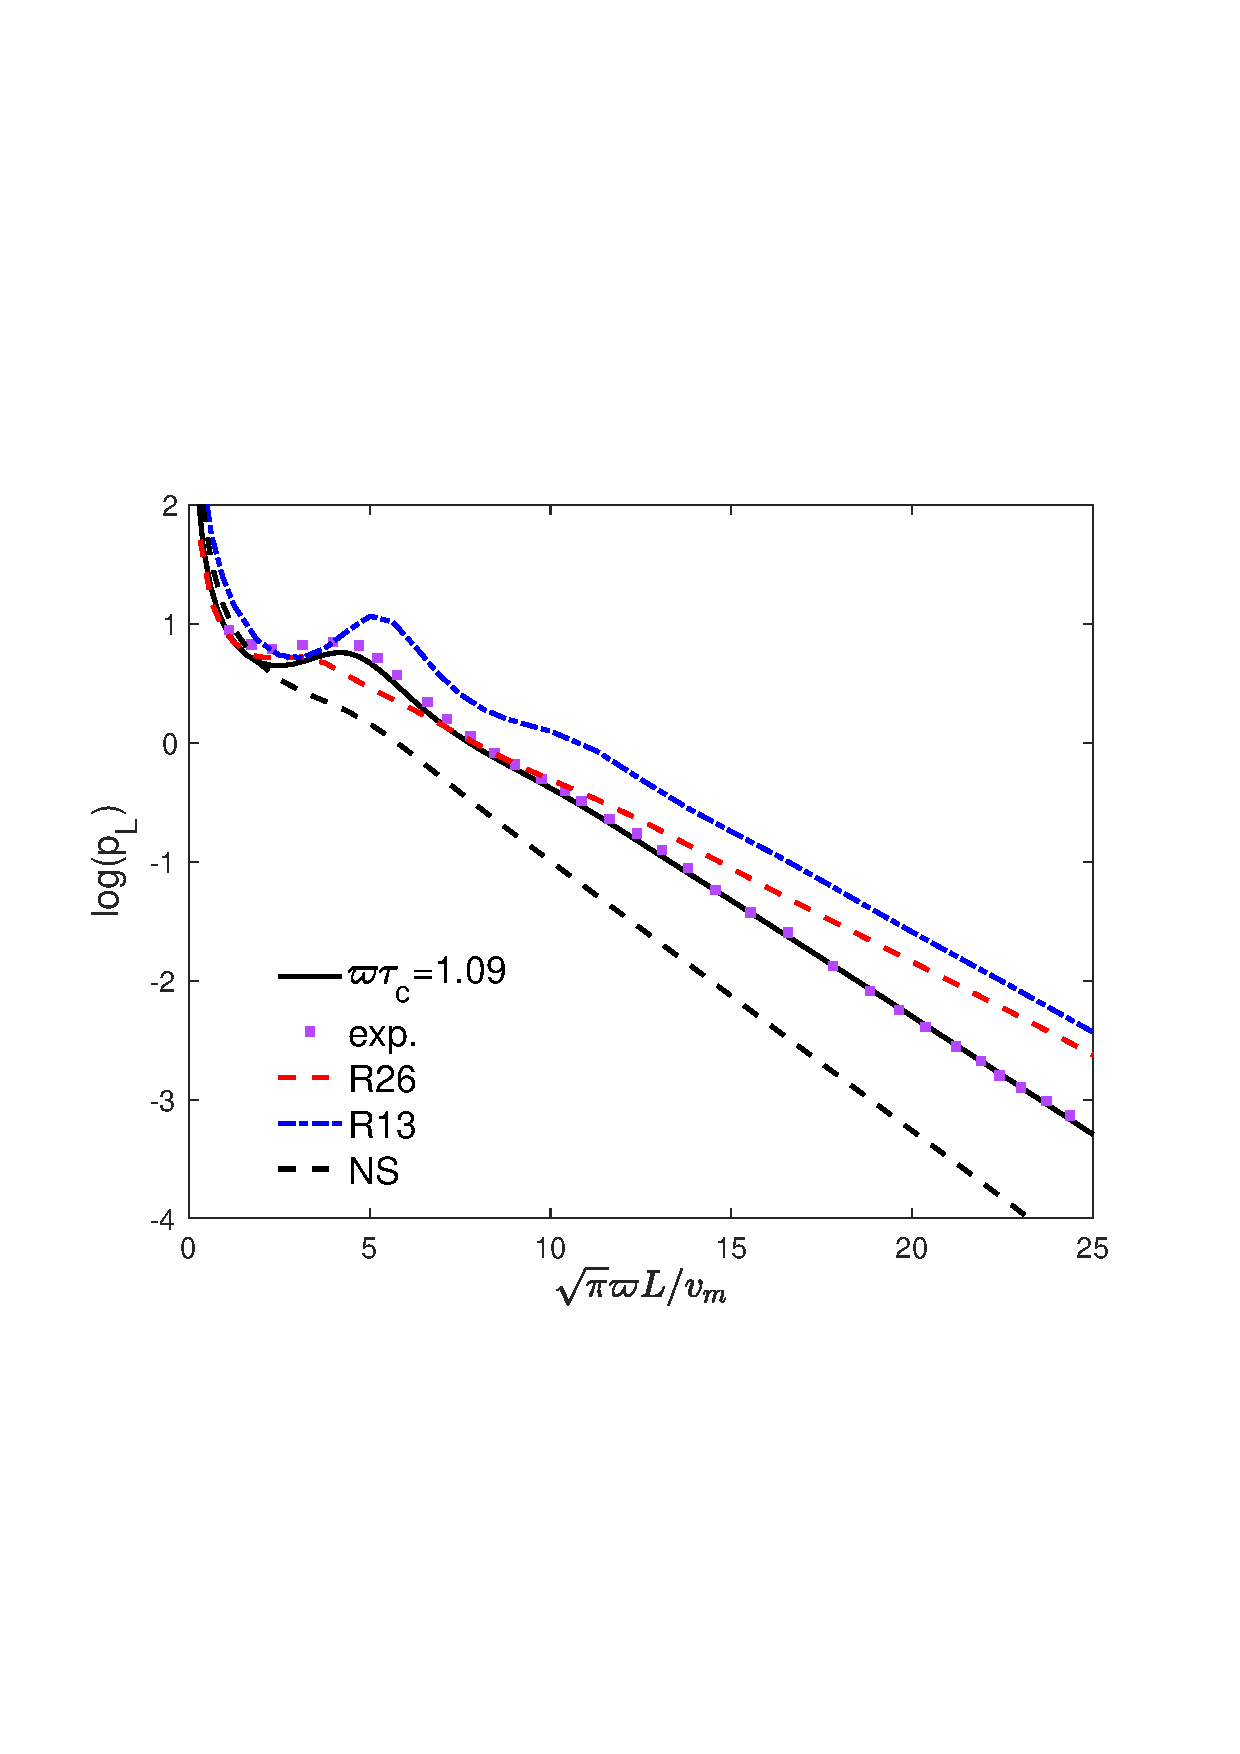
\includegraphics[width=0.45\textwidth]{Introduction/IMG/testOmgTau1_09.pdf}
	\caption{ 
		(Top) Sound propagation between transducer and receiver. (Bottom) Dimensionless sound amplitude $p_L$ at the receiver as a function of the dimensionless length $\sqrt\pi\varpi{L}/v_m$, where $\varphi$ is the sound frequency and $v_m$ is the most probable speed of gas molecules. Experimental data are collected from Ref.~\cite{Schotter1974} when the gas medium is helium. Solid lines represent the numerical solutions of the Boltzmann equation with the diffuse boundary condition~\cite{Wu2020AIA}. R13 and R26: the regularized 13 and 26 moment equations derived from the Boltzmann equation, which are more accurate than the NSF equations.
	 } %where $p_L$ is normalized by $pu_w/v_m$, with $p$, $u_w$ and $v_m$ being the gas pressure, velocity amplitude of the transducer and most probable speed, respectively
	\label{fig:sound}
\end{figure}




% ~\cite{Beskok_book} %An important research topic is to investigate the damping force that any oscillatory parts are subject to, which has applications in inertial sensing and acoustic transduction. %The normal pressure and shear force from the ambient gas damp the vibrating devices; 

The rarefied gas flow at the micro-scale has a broad range of industrial applications, and has attracted particular attention due to the rapid development of microelectromechanical systems~\cite{Beskok_book}. At small length scale, and sometimes the high oscillation frequency, the NSF equations loss validity.

\index{sound wave}
\index{oscillation frequency}

Figure~\ref{fig:sound} shows the sound resonance between the transducer and receiver, where the sound pressure at the receiver is a function of the oscillation frequency $\varpi$ and propagation distance $L$. When $\varpi$ is 0.3 times of the mean collision frequency of gas molecules $\bar{\nu}$,
\begin{equation}\label{chapter1_tau_c}
\bar{\nu}=\frac{1}{\tau_c}=\frac{p}{\mu},
\end{equation}
the NSF equations fail to predict the sound pressure at the receiver; other high-order macroscopic equations, like the regularized 13 and 26 moment equations derived from the Boltzmann equation~\cite{henning,Gu2009JFM}, however, can well predict the sound pressure. When $\varpi$ is increased to $1.09\bar{\nu}$, the difference between NSF predictions and experimental data further enlarges, and regularized 13 and 26 moment equations fail too. However, the Boltzmann equation predicts the sound pressure well~\cite{Wu2020AIA}.


\textbf{声波中的自由度冻结}

\begin{figure}[t]
	\centering
	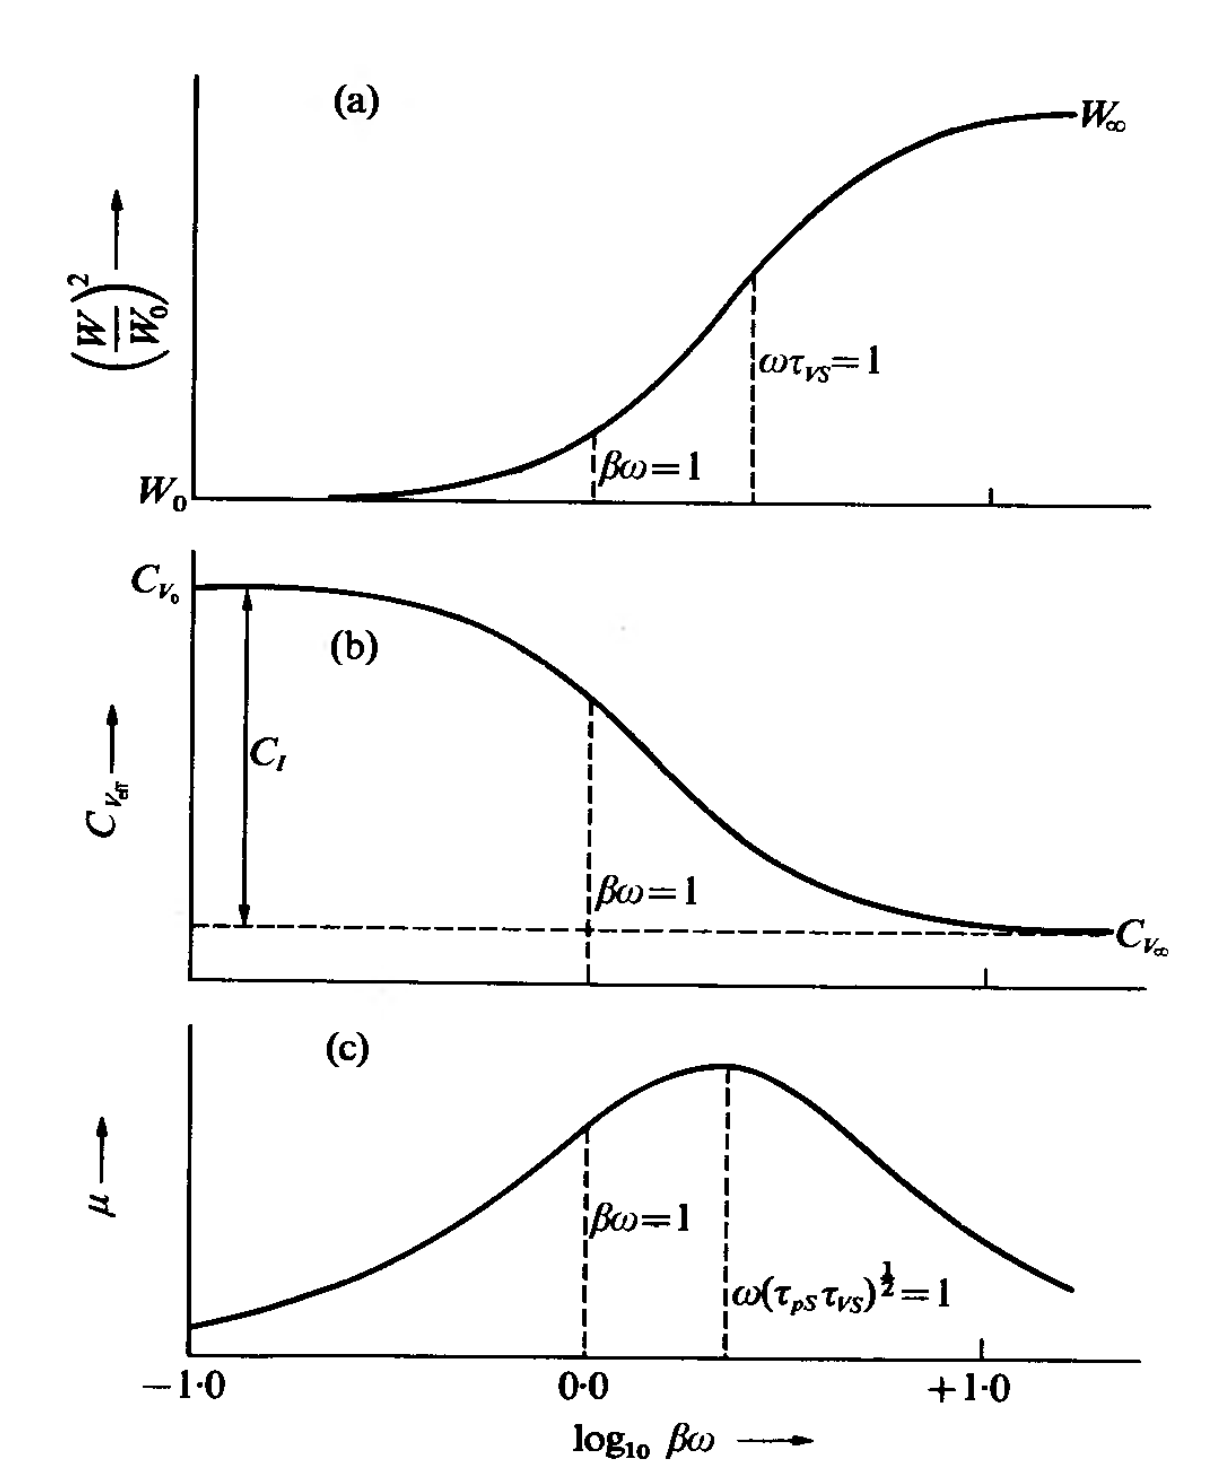
\includegraphics[width=0.6\textwidth]{Introduction/IMG/frozen_sound_demo.png}
	\caption{ 
	声波中的等效声速、等容热容和衰减率随声波频率的变化关系 \cite{Lambert1977}。
	} %where $p_L$ is normalized by $pu_w/v_m$, with $p$, $u_w$ and $v_m$ being the gas pressure, velocity amplitude of the transducer and most probable speed, respectively
	\label{fig:sound_frozen}
\end{figure}



\subsection{Shale gas extraction}
\index{shale gas extraction}
\index{dense gas}

\begin{figure}[t]
	\centering
	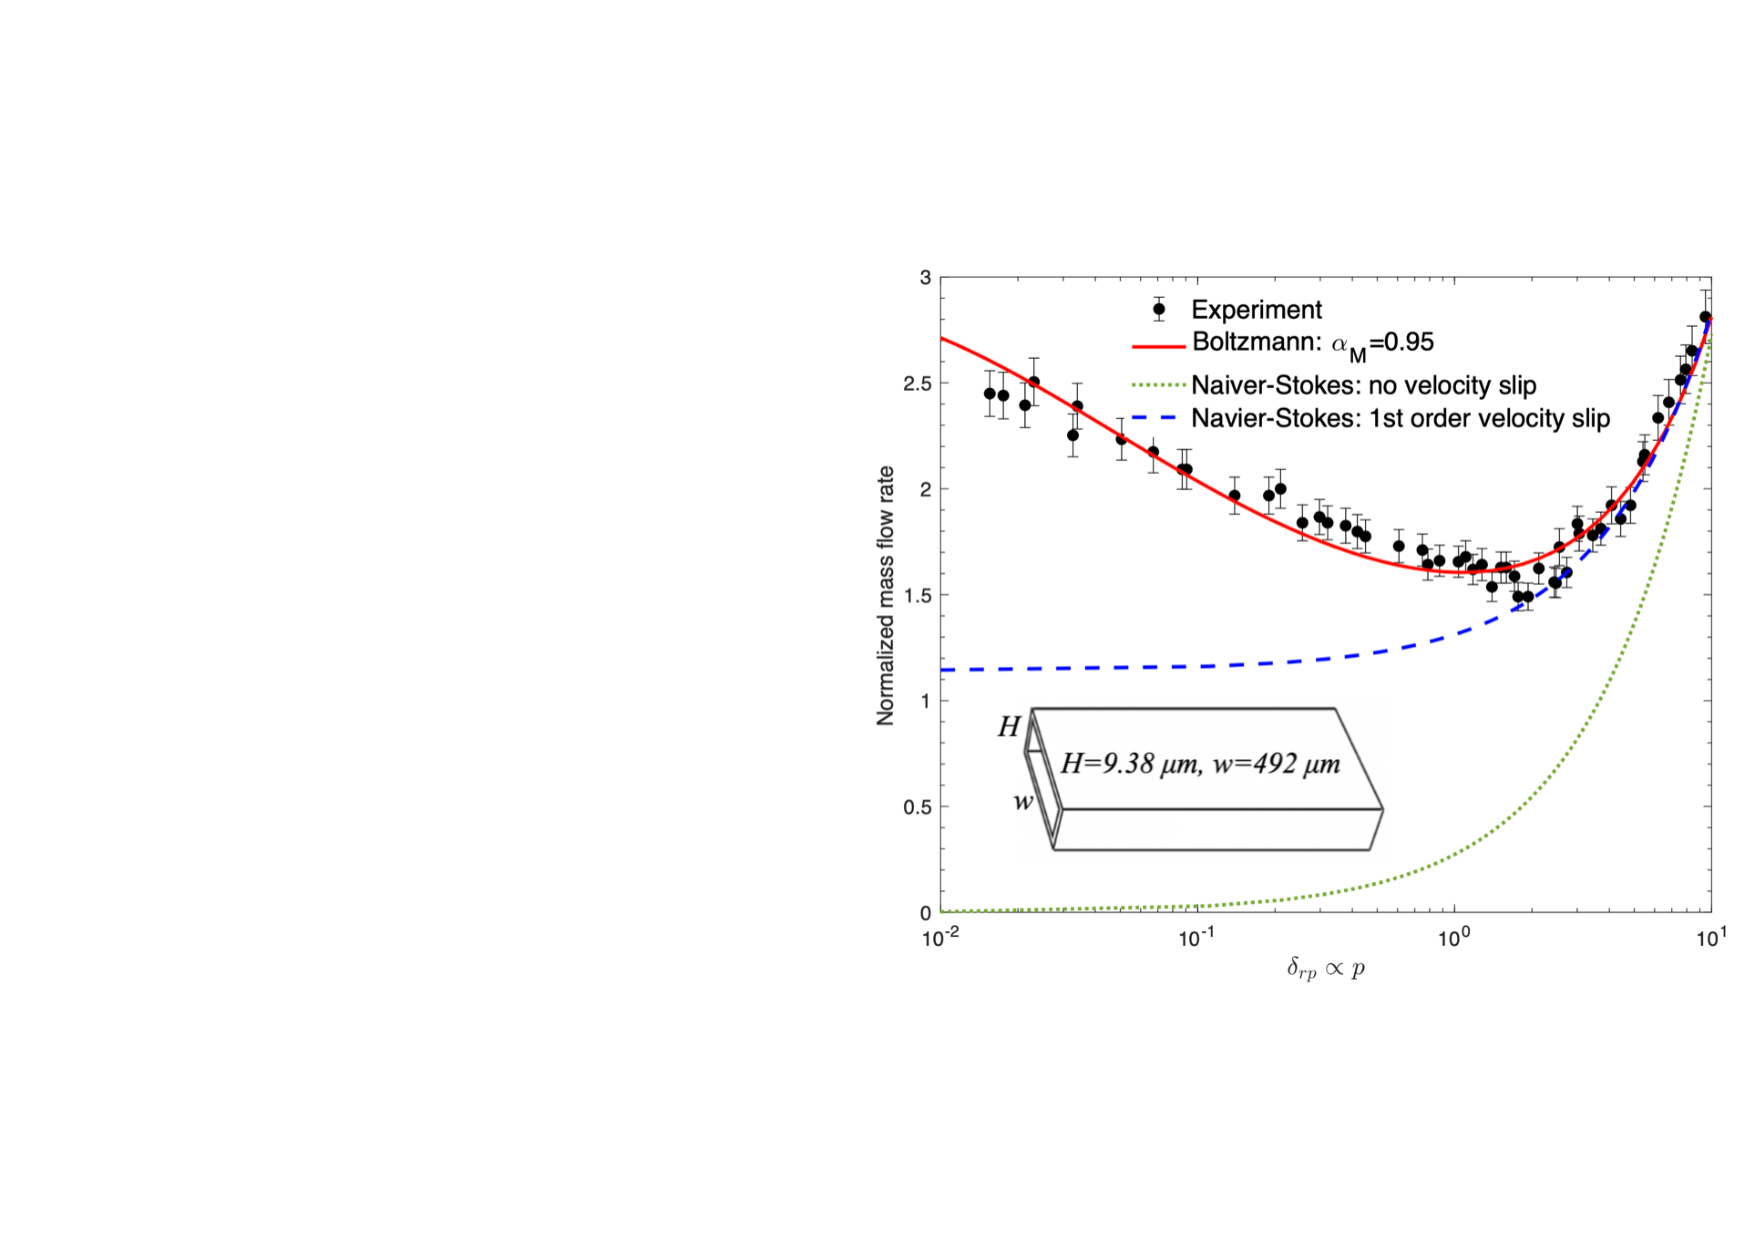
\includegraphics[width=0.6\columnwidth]{Introduction/IMG/CSG.pdf}
	\caption{ The normalized mass flow rate as a function of the rarefaction parameter~\eqref{rarefaction_chapter1_parameter}, for the gas flow through a long and narrow duct~\cite{Ewart2007,WuStruchtrupJFM2017}. 
}
	\label{ShaleGasExtracton}
\end{figure}


Unconventional gas reservoirs have attracted significant attention due to the shale gas revolution, but the accurate prediction of gas production is a grand research challenge. In shale gas exploitation, the gas pressure could reach hundreds times of atmospheric pressure, but the flow passage is at the nanometer scale. Although the gas is dense~\cite{Lei2015Enskog,Wu2016JFM}, its flow dynamics can still be rarefied\footnote{The antonym of ``dense gas'' is ``dilute gas'', while the ``rarefied gas'' is referred to the gas in which the flow cannot be adequately described by NSF equations.}. Experimental data on gas flow through  porous media is hard to measure and interpret, so we introduce the experiment of micro gas flow to demonstrate the influence of rarefaction effects~\cite{Ewart2007}.


The duct shown in the inset of Fig.~\ref{ShaleGasExtracton} has a cross-section dimension of 9.38 $\mu$m $\times$ 492 $\mu$m, which is connected to two large reservoirs at the ends. Given the inlet and outlet pressures ($p_{in}$ and $p_{out}$, respectively), the mass flow rate (MFR, $\dot{M}$) is measured when the steady-state of the flow is reached. Then the normalized MFR \index{mass flow rate}
\begin{equation}
	G=\frac{L\sqrt{2k_BT_0/m}}{H^2w(p_{in}-p_{out})}\dot{M},
\end{equation}
is plotted against the mean gas pressure $p$. At large gas pressures the NSF equations predict the MFR well. However, when the gas pressure is reduced, the normalized MFR predicted by NSF equations always decreases, while that from the experiment first decreases and then increases, resulting in the famous phenomenon of \index{Knudsen minimum} ``Knudsen minimum''. At low pressures, the NSF equations could underpredict the MFR by several orders of magnitude; even with the correction of wall slip velocity, they underpredict the MFR by several times.  


\begin{figure}[t]
	\centering
	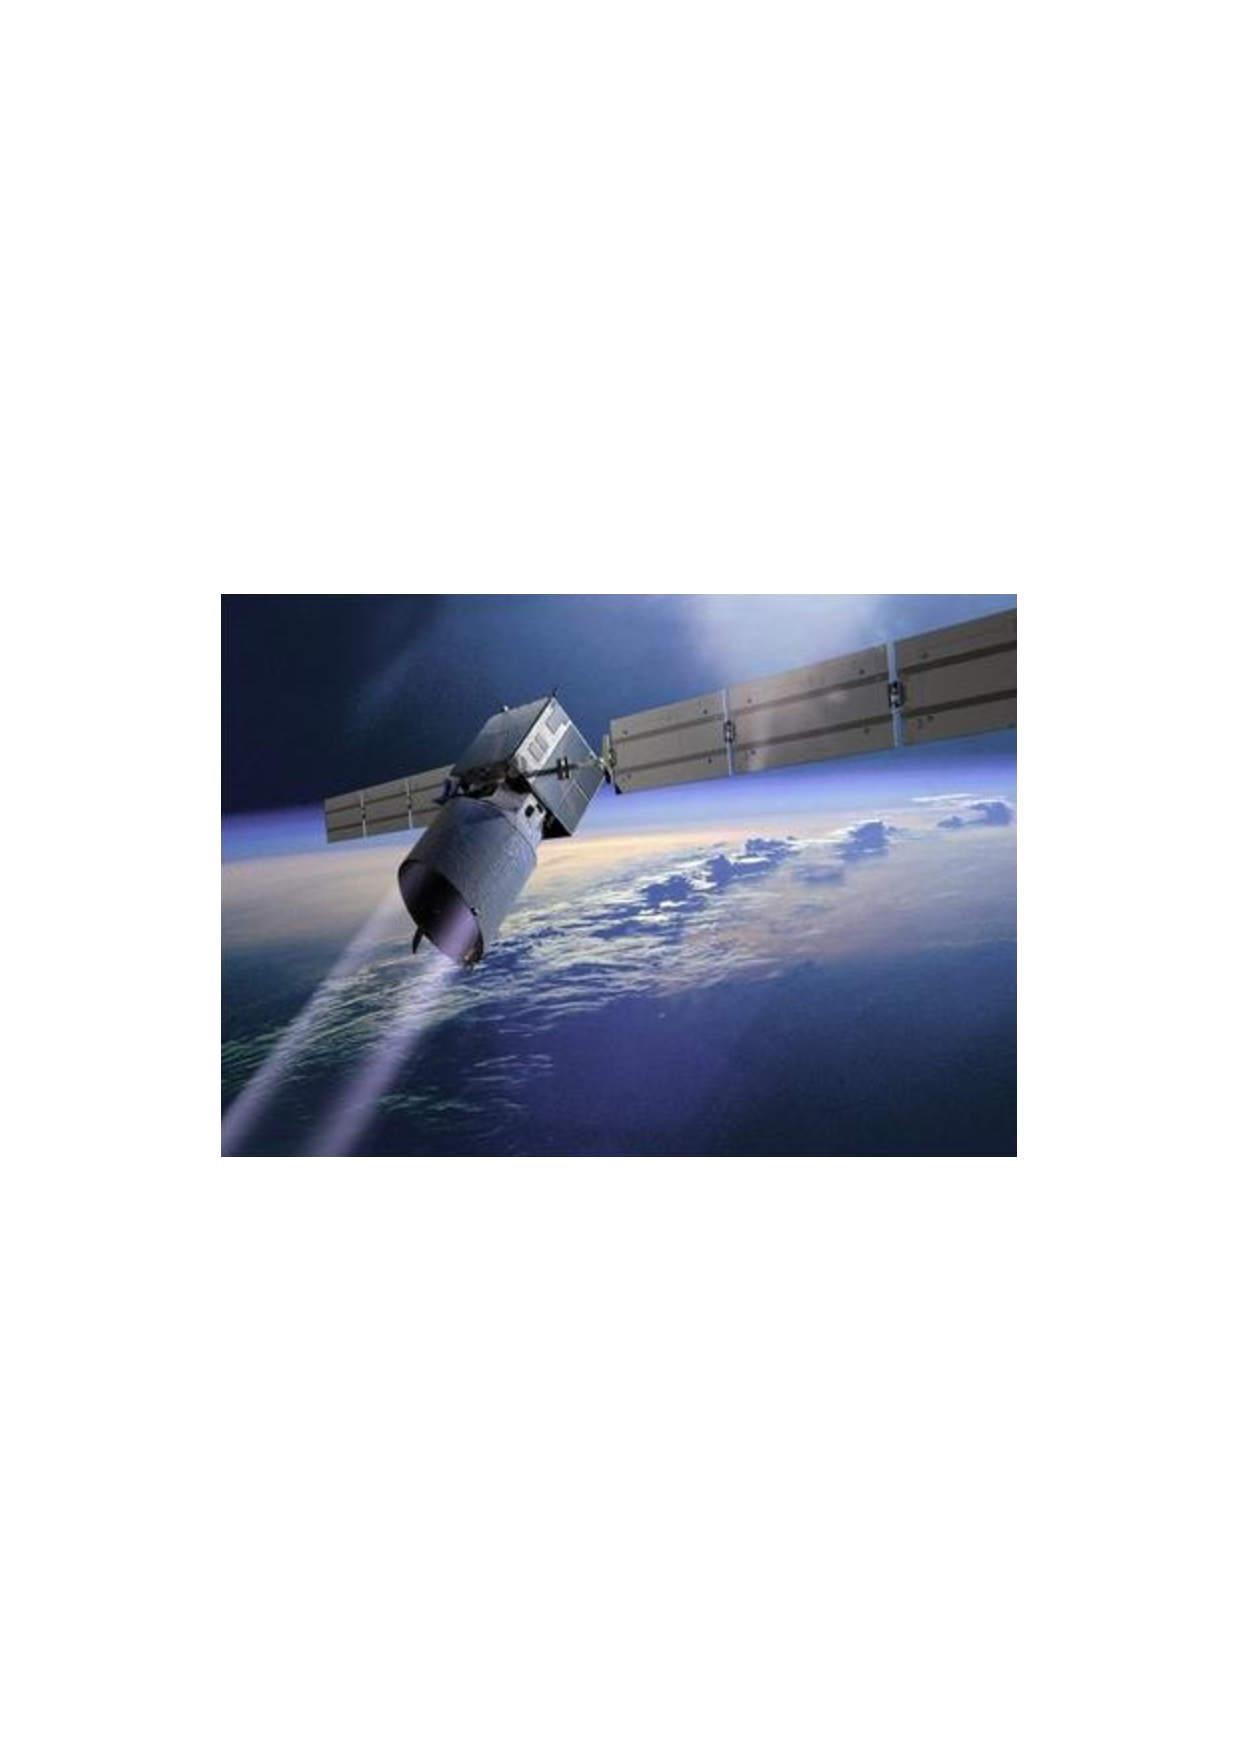
\includegraphics[width=0.45\columnwidth]{Introduction/IMG/ESA_gallery}
	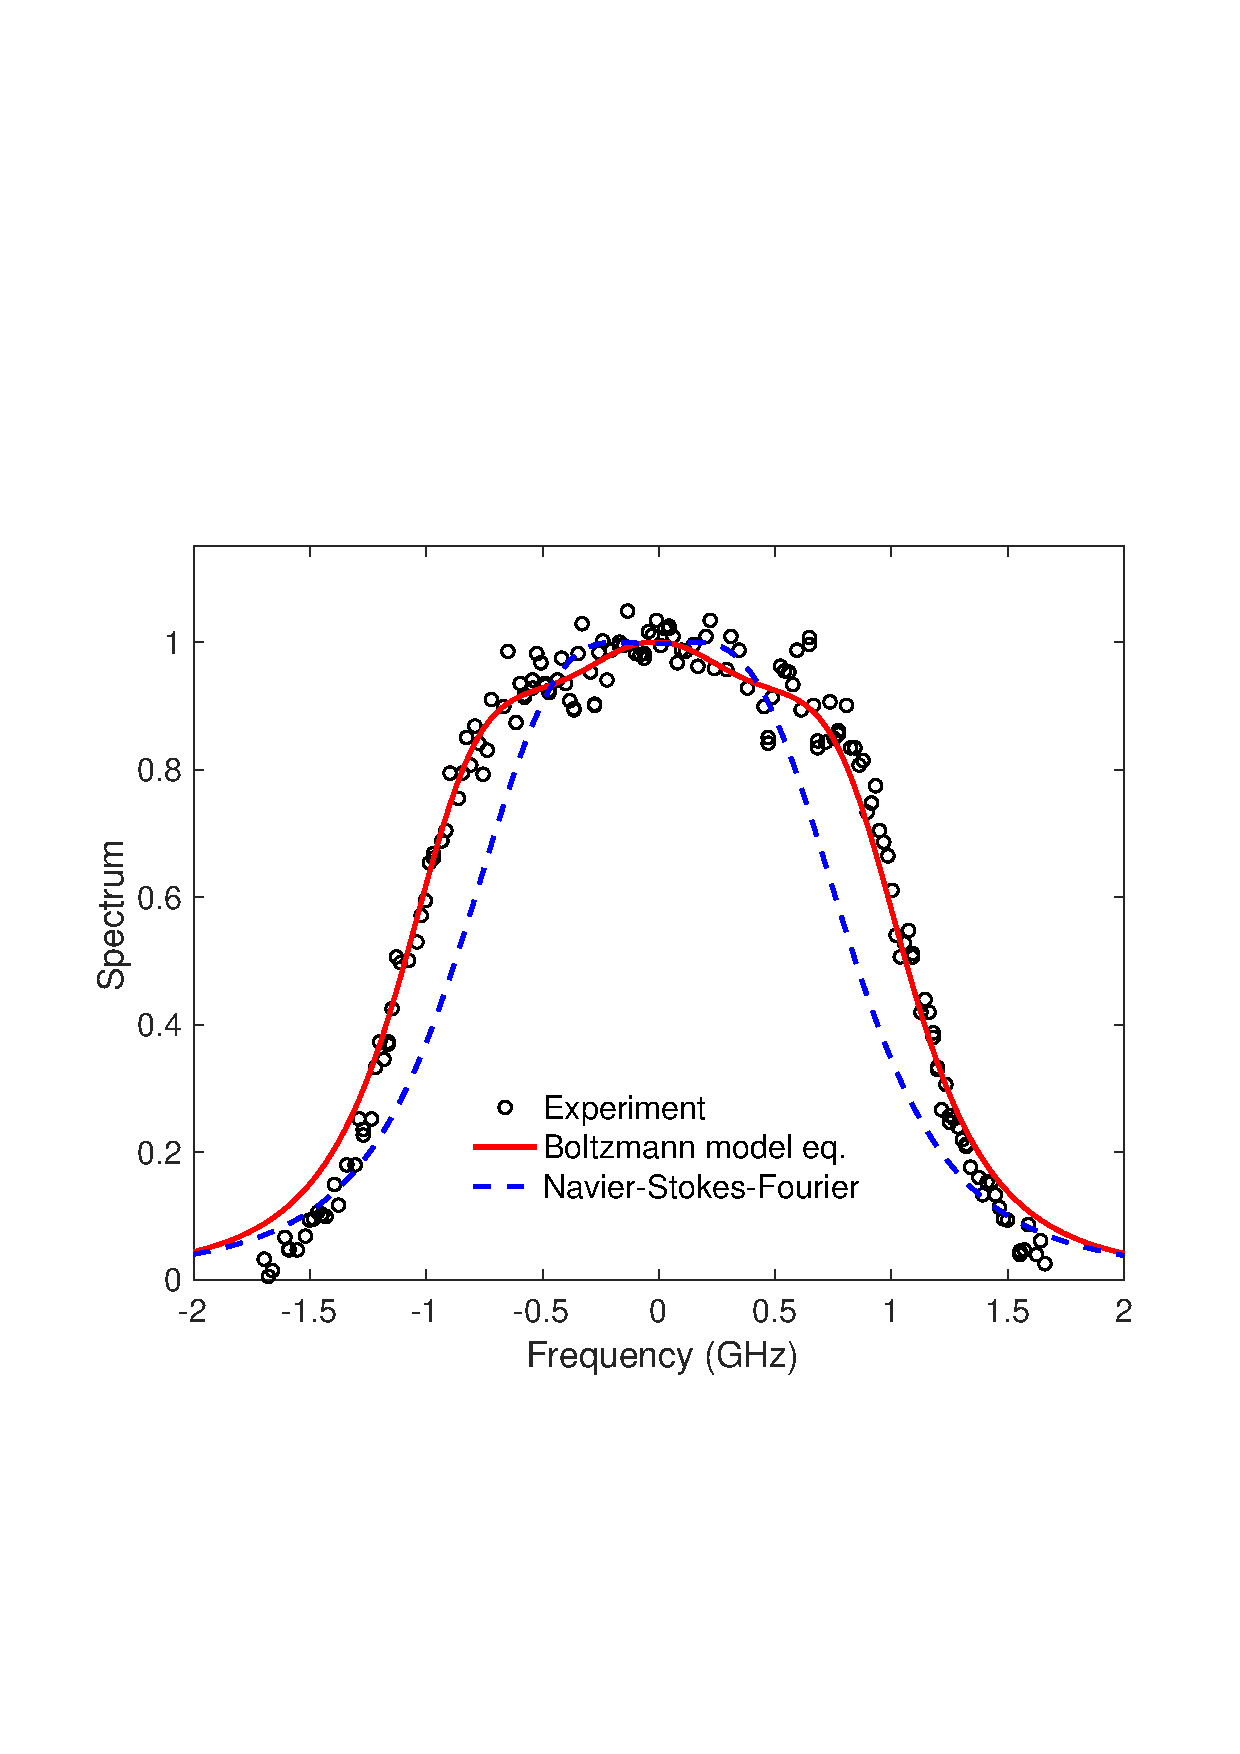
\includegraphics[width=0.5\columnwidth]{Introduction/IMG/PRL2}
	\caption{ 
		Comparisons in the spectra of spontaneous Rayleigh-Brillouin scattering \index{Rayleigh-Brillouin scattering} between the experimental data~\cite{Greytak1966PRL}, the linearized Boltzmann equation~\cite{Wu2020AIA} (see Chapter~\ref{chap:fluctuation}), and the NSF equations. The light is scattered from CO$_2$ with zero flow velocity, at a pressure of 770 mm of Hg. The Knudsen number~\eqref{Kn_original} is $\text{Kn}=0.14$. 
	}
	\label{AdmAeolus}
\end{figure}



\subsection{Global wind profiling}\label{ADM_aeolus}

% \footnote{ADM stands for Atmospheric Dynamics Mission, while in the works of the Greek poet Homer, Aeolus is the controller of the winds and ruler of the floating island of Aeolia.}

In 2018, the European Space Agency launched the satellite ADM-Aeolus to measure the global wind profile for an improved understanding of atmospheric dynamics. The ADM-Aeolus mission makes use of the Doppler Wind Lidar measurement technique, and the spectrum of scattered light is important for the accurate retrieval of wind profile. Due to the high scattering frequency and short laser wavelength, as compared respectively to the mean collision frequency and mean free path of gas molecules, the gas dynamics is not in equilibrium, and the NSF equations have large error, see Fig.~\ref{AdmAeolus}.



%the measurement data will allow achievement of the  goals of Aeolus:
%\begin{itemize}
%	\item Provision of accurate wind profiles throughout the troposphere and lower stratosphere eliminating a major deficiency in the Global Observing System.
%	
%	\item Provision of data for the study of global atmospheric circulation and related features, such as precipitation systems, the El Niño and the Southern Oscillation phenomena and stratospheric/tropospheric exchange.	
%		
%	\item  Validate climate models through the use of high quality wind profiles from a global measurement system.
%		
%	\item  Improve understanding of atmospheric dynamics and the global atmospheric transport and cycling of energy, water, aerosols, chemicals and other airborne materials.
%		
%%	\item  Generate a number of derived products such as cloud top altitudes, aerosol properties and tropospheric height.	
%\end{itemize}






\section{Simple gas kinetic theory}\label{simple_kinetic_theory}
\index{simple gas kinetic theory}

The breakdown of NSF constitutive relations may be understood qualitatively from the simple kinetic theory, which not only allows the estimation of transport coefficients \index{transport coefficient} such as the shear viscosity, thermal conductivity and self-diffusion coefficient, but also indicates the origin of rarefaction effects. 

Consider a gas of hard-spheres (HS) \index{hard sphere} of diameter $\sigma$ and number density $n$, traveling with the average speed $\bar{c}$. Imagine a gas molecule moves through the gas with the average relative speed $\sqrt{2}\bar{c}$, while other molecules are fixed. During the time interval $\Delta{t}$ the moving molecule sweeps a volume of $\Delta{V}=\sqrt{2}\pi\sigma^2\bar{c}\Delta{t}$, which encounters collisions with $n\Delta{V}$ molecules. Hence the average time for one collision is $\tau_c={1}/{\sqrt{2}n\pi\sigma^2\bar{c}}$,
and the MFP is \index{mean free path}
\begin{equation}\label{mfp_hs}
\lambda=\bar{c}\tau_c=\frac{1}{\sqrt{2}n\pi\sigma^2}.
\end{equation}

In simple kinetic theory it is assumed that one sixth of the molecules moves into each of the 6 directions of space, and within one mean free path there are no collisions among gas molecules (hence it can be derived from the ideal gas law $p=nk_BT$ that the average speed is $\bar{c}=\sqrt{{3k_BT}/{m}}$). 
Therefore, the number flux (the number of gas molecules per unit area per unit time) through a plane perpendicular to the $x_1$-axis is 
\begin{equation}\label{simple_kinetic1}
J_1=\frac{n(x_1-\lambda)}{6}\bar{c}-\frac{n(x_1+\lambda)}{6}
\approx -\frac{\bar{c}}{3}\lambda\frac{dn}{dx_1}.
\end{equation}
Similarly, the shear stress (momentum flux) and heat flux (due to the translational motion only) are
\begin{equation}\label{simple_kinetic2}
\begin{aligned}[b]
\sigma_{12}=\frac{mn\bar{c}}{6}
\left[
u_2(x_1-\lambda)-u_2(x_1+\lambda)
\right]
\approx-\frac{mn\bar{c}}{3}\lambda\frac{\partial u_2}{\partial x_1},\\
q_{1}=\frac{mn\bar{c}}{6}
\left[\frac{3}{2}\frac{k_B}{m}T(x_1-\lambda)
-\frac{3}{2}\frac{k_B}{m}T(x_1+\lambda)\right]
\approx-\frac{nk_B\bar{c}}{2}\lambda\frac{\partial T}{\partial x_1},
\end{aligned}
\end{equation}
therefore the diffusion coefficient, shear viscosity, and thermal conductivity are respectively
\begin{equation}
\begin{aligned}
D=\frac{\bar{c}}{3}\lambda,\quad
\mu=\frac{mn\bar{c}}{3}\lambda, \quad
\kappa=\frac{nk_B\bar{c}}{2}\lambda.
\end{aligned}
\end{equation}

\index{shear viscosity}
\index{thermal conductivity}
\index{diffusion coefficient}

It is clear from Eqs.~\eqref{simple_kinetic1} and~\eqref{simple_kinetic2} that these transport coefficients are derived only when the first-order Taylor expansion is used; this requires the fluid system varies slowly on a spatial scale of the size of MFP, otherwise higher-order expansions are needed, and the constitutive relations will go beyond Newton's law of stress and  Fourier's law of heat conduction. Therefore, the degree of rarefaction effects can be characterized by the ratio of mean free path to the characteristic flow length in which the macroscopic quantities vary.  
\index{Newton's law of stress}
\index{Fourier's law of heat conduction}

%Similarly, the heat flux due to the translational and internal motion of gas molecules (with degrees of freedom being $d_t=3$ and $d_i$, respectively) are
%\begin{equation}
%\begin{aligned}
%q_{tra}=\frac{mn\bar{c}}{6}
%\left[\frac{d_t}{2}\frac{k_B}{m}T(x_1-\lambda)
%-\frac{d_t}{2}\frac{k_B}{m}T(x_1+\lambda)\right]
%\approx-\frac{nk_Bd_t\bar{c}}{6}\lambda\frac{\partial T}{\partial x_1},\\
%q_{rot}=\frac{mn\bar{c}}{6}
%\left[\frac{d_i}{2}\frac{k_B}{m}T(x_1-\lambda)
%-\frac{d_i}{2}\frac{k_B}{m}T(x_1+\lambda)\right]
%\approx-\frac{nk_Bd_i\bar{c}}{6}\lambda\frac{\partial T}{\partial x_1},
%\end{aligned}
%\end{equation}
%which means that the translational and internal thermal conductivities are
%\begin{equation}
%\kappa_{tra}=\frac{nk_Bd_t\bar{c}}{6}\lambda, \quad
%\kappa_{rot}=\frac{nk_Bd_i\bar{c}}{6}\lambda.
%\end{equation}

%Therefore, we have 
%\begin{equation}
%{\kappa_{rot}}=\frac{\mu{}k_Bd_i}{2m}\times\frac{\rho{}D}{\mu}=\frac{\mu{}k_Bd_i}{2m}\times\frac{1}{\text{Sc}}. 
%\end{equation}
%
%From equation (2.4) we know that, if there is no cross exchange coefficients, we have  
%\begin{equation}
%\kappa_{rot}=\frac{\mu{}k_B{d_i}}{2m}\times\frac{1}{A_{rr}}.
%\end{equation}

\section{Knudsen number}
\index{Knudsen number}

The RGD emerges in extreme conditions where the gas density is low, the characteristic flow length is small, and/or when the oscillation frequency is high. This brings us to the introduction of dimensionless parameter, the Knudsen number, to approximately measure the degree of non-equilibrium. 



\subsection{Spatial Knudsen number}
\index{Knudsen number! spatial}

The Knudsen number,  defined as the ratio of the molecular MFP $\lambda$ to the characteristic flow length $L$, is widely used:
\begin{equation}\label{Kn_original}
\text{Kn}=\frac{\lambda}{L}, 
\end{equation} 
where the MFP \index{mean free path} can be defined in terms of the shear viscosity as
\begin{equation}
\lambda=\frac{\mu}{p}\sqrt{\frac{\pi{}k_BT_0}{2m}},
\end{equation} 
rather than Eq.~\eqref{mfp_hs} that is derived from the simple kinetic theory based on HS molecular model. This is obvious because for other types of intermolecular potential it is difficult to determine the molecular diameter. 


This Knudsen number is known as the spatial Knudsen number as spatial length scales are involved. Note that sometimes the rarefaction parameter, \index{rarefaction parameter} which is inversely proportional to the spatial Knudsen number, is used instead:
\begin{equation}\label{rarefaction_chapter1_parameter}
\delta_{rp} =\frac{pL}{\mu{v_m}}=\frac{\sqrt{\pi}}{\text{2Kn}}.
\end{equation}
This parameter appears in the kinetic model equations when the Boltzmann collision operator is simplified. 

\begin{figure}[t]
	\centering
	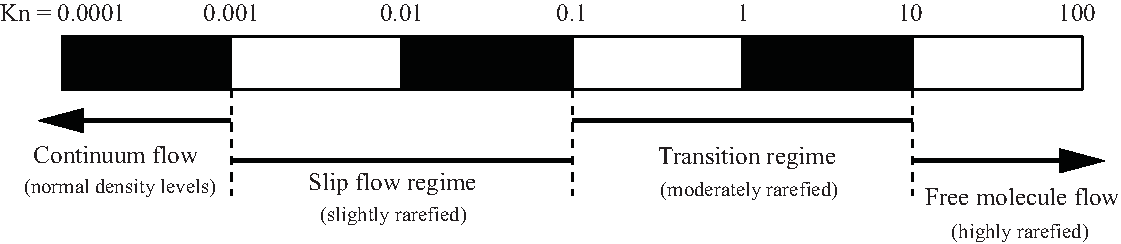
\includegraphics[scale=0.7]{Introduction/IMG/Kn.pdf}\\
	\caption{
		Flow regime classification based on the spatial Knudsen number~\cite{Qian1946,Gad-el-Hak1999}.}
	\label{Kn_region}
\end{figure}

As shown in Fig.~\ref{Kn_region}, the spatial Knudsen number is used to classify the gas flow into four regimes~\cite{Qian1946,Gad-el-Hak1999}: \index{flow regime}
\begin{itemize}
	\item Continuum flow regime. \index{continuum flow} When $\text{Kn}\lesssim0.001$, the NSF equations with the non-velocity-slip and non-temperature-jump boundary conditions are adopted to describe the gas dynamics\footnote{There are some exceptions, where the NSF equations do not describe the gas dynamic accurately even when $\text{Kn}$ approaches zero. For example, the ghost effect induced by the periodical variation of wall temperature~\cite{Sone2002Book}.}. 
	
	\item Slip flow regime. \index{slip flow}  When $0.001\lesssim{}\text{Kn}\lesssim0.1$,  weak rarefaction effects such as the velocity slip and temperature jump emerge in the Knudsen layer, i.e., a small region within a few MFP away from the solid wall. With appropriate velocity-slip and temperature-jump boundary conditions, the NSF equations may still produce reasonable results. 
	
	\item  Transition flow regime. \index{transition flow} When $0.1\lesssim{}\text{Kn}\lesssim10$, strong rarefaction effects modify the constitutive relations as assumed in continuum mechanics so that the NSF equations break down completely, and gas-kinetic equations such as the Boltzmann equation is used to describe rarefied gas flows~\citep{CE}. 
	
	\item Free-molecular flow regime. \index{free-molecular flow} When $\text{Kn}\gtrsim10$, the collision between gas molecules do not play an important role, while the collision between the gas and wall molecules (gas-surface interaction) is dominant.
	
\end{itemize}

\begin{figure}[t]
	\centering
	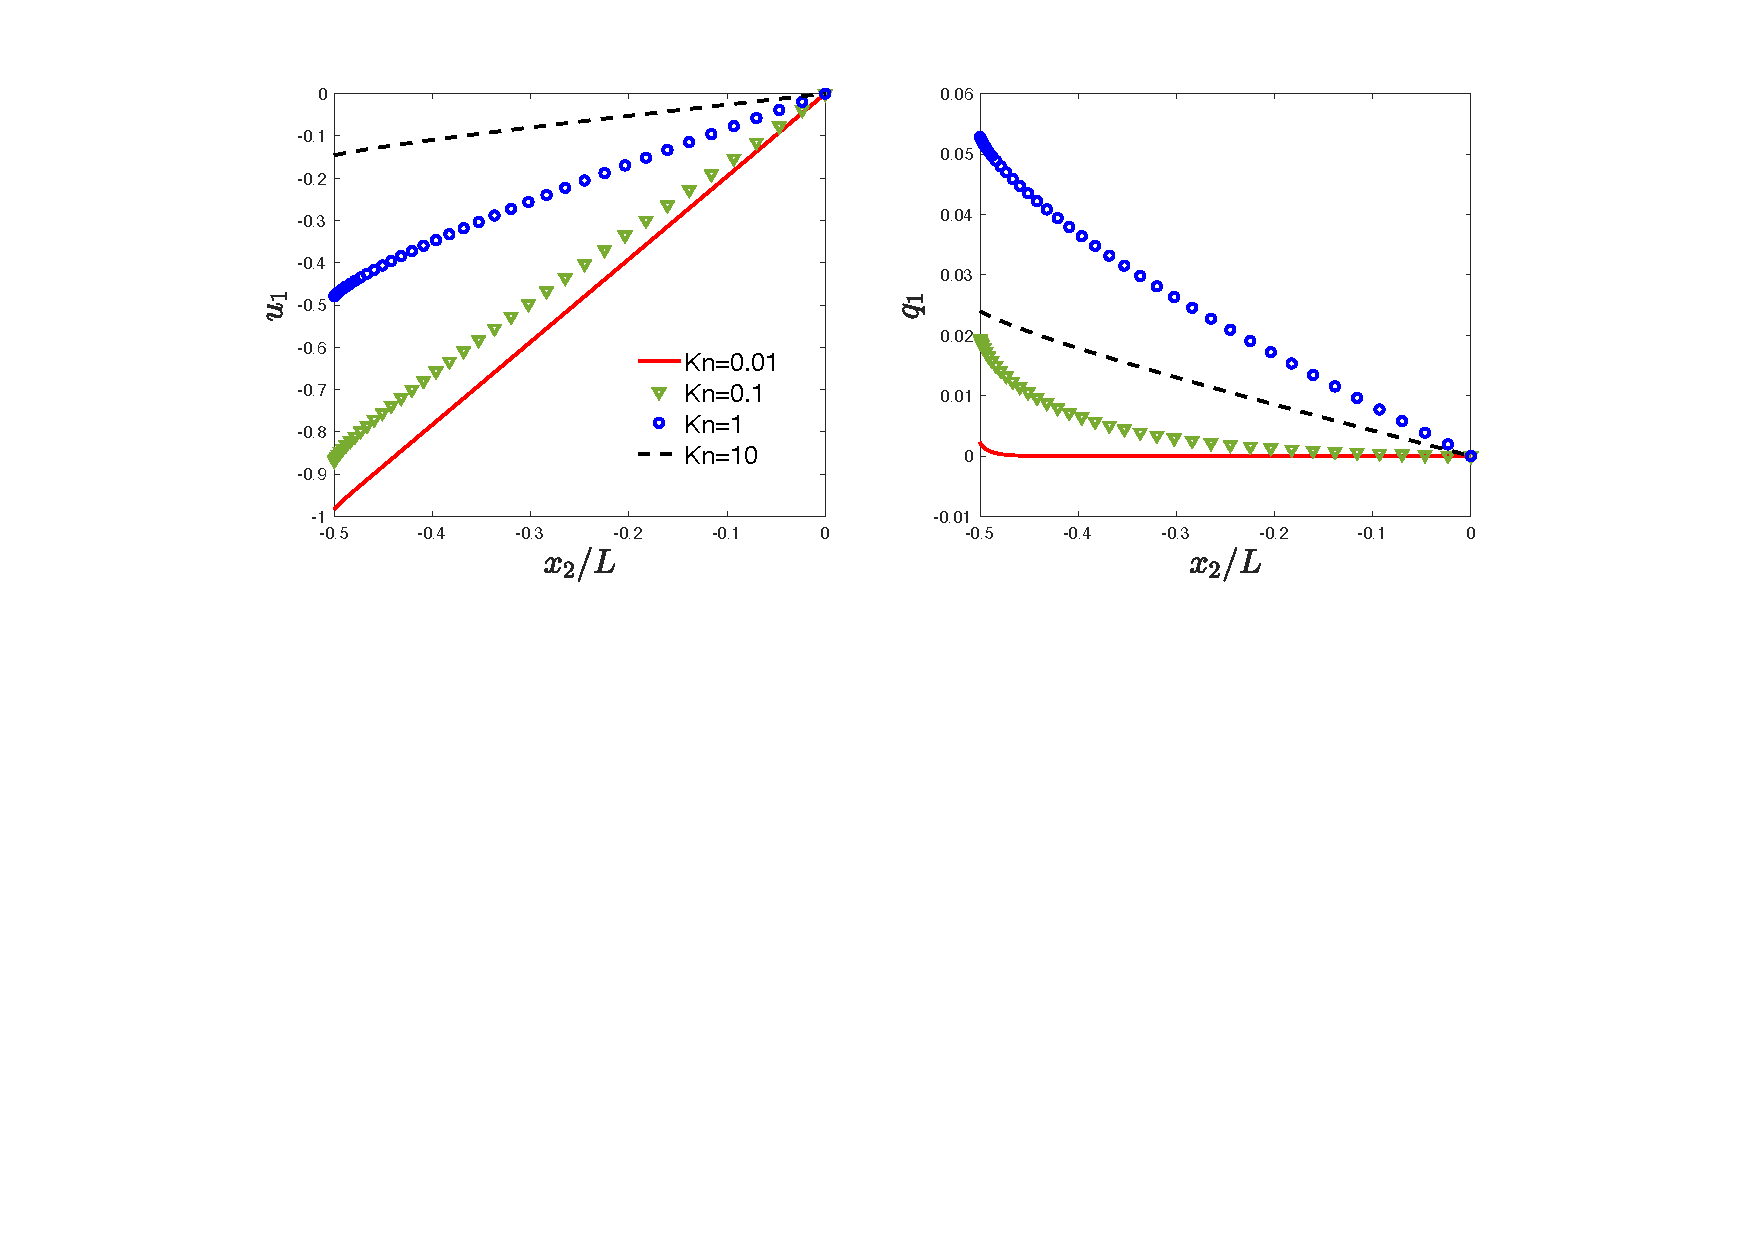
\includegraphics[scale=0.7]{Introduction/IMG/Couette_Route_NonEquilibrium2.pdf}\\
	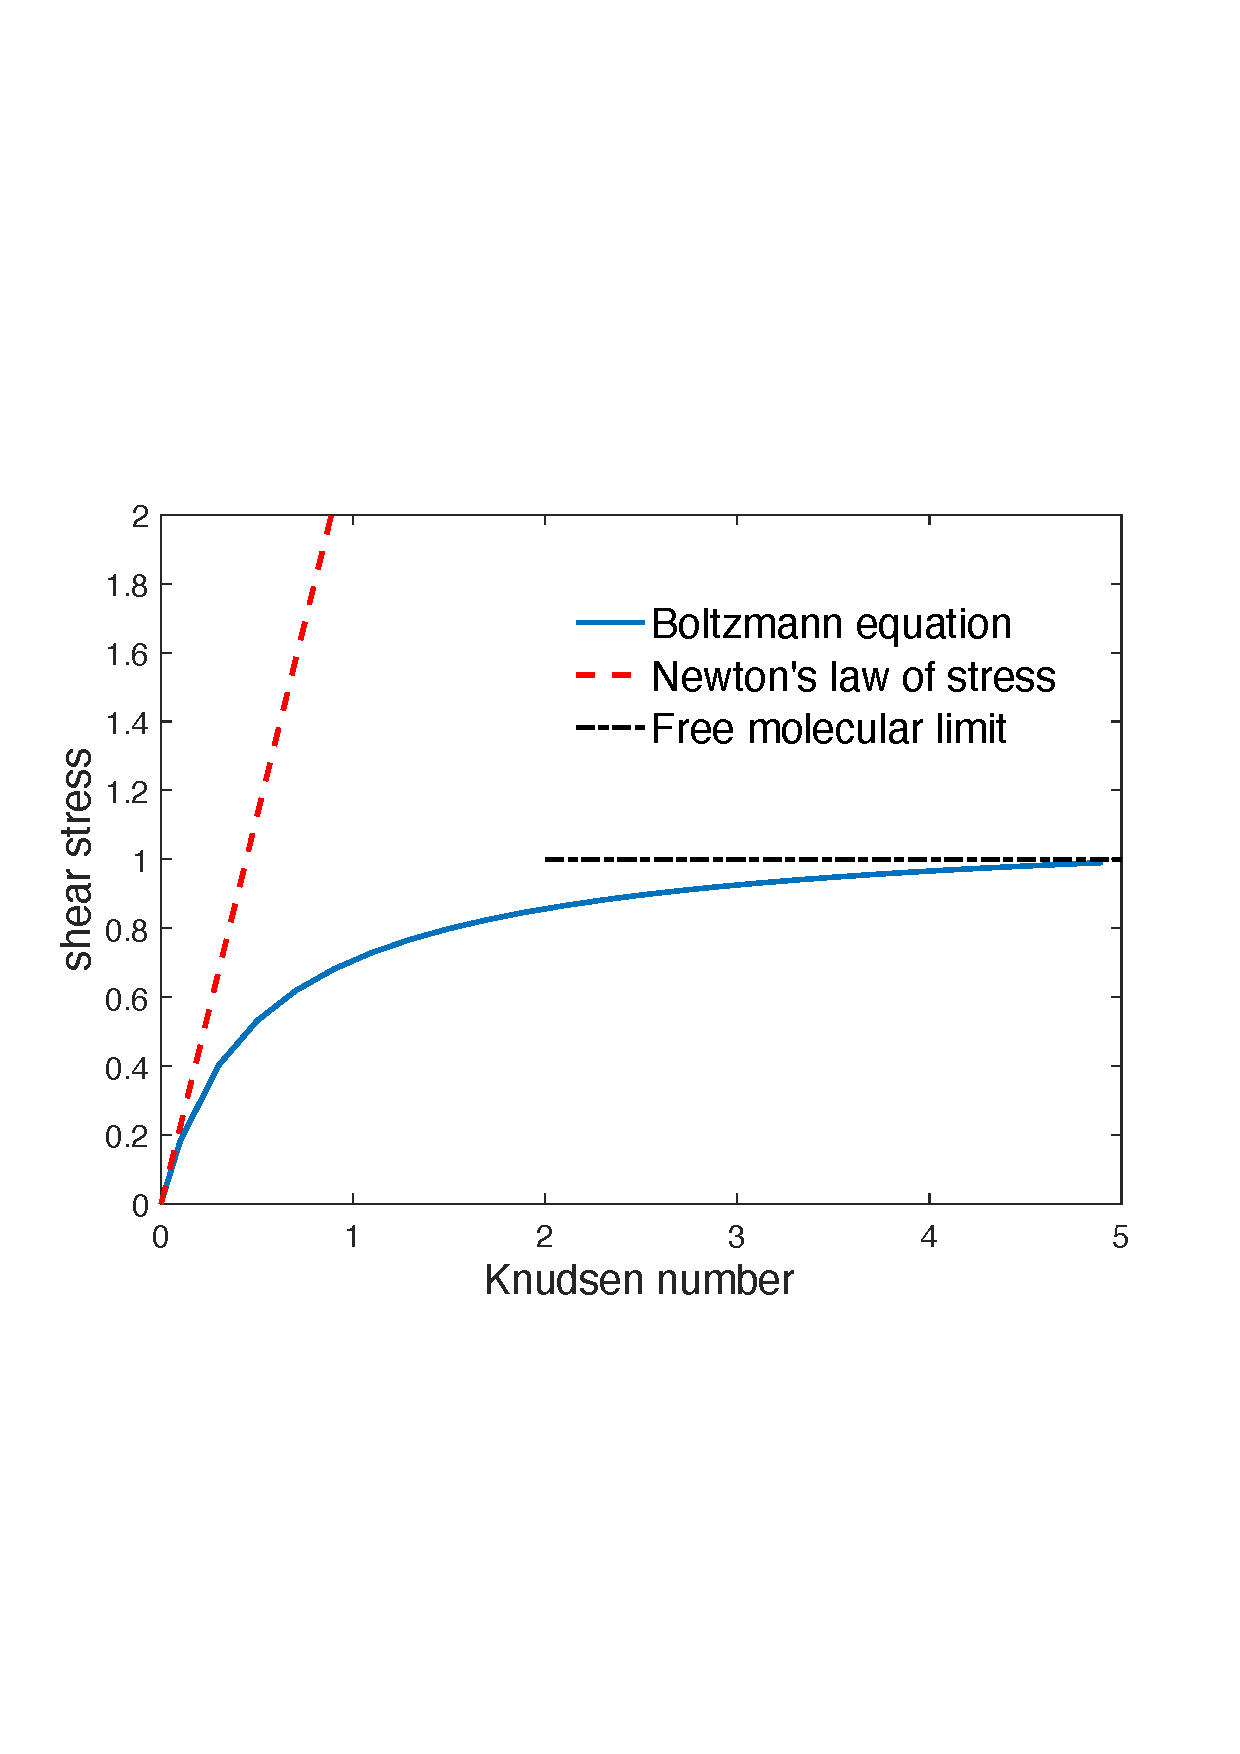
\includegraphics[scale=0.4]{Introduction/IMG/shearStress_Couette2.pdf}
	\caption{
		The flow velocity (normalized by wall velocity), heat flux (normalized by the product of gas pressure and wall velocity), and shear stress (normalized by the product of gas pressure and dimensionless velocity $u_w/\sqrt{2k_BT_w/m}$)  of the planar Couette flow at different values of spatial Knudsen number, obtained from the linearized Boltzmann equation for HS gas with the diffuse boundary condition.}
	\label{Kn_region_couette}
\end{figure}


\textbf{Route to nonequilibrium}---We take the planar Couette flow \index{Couette flow} as an example to demonstrate how the rarefaction effects set in. Consider two parallel plates located  at $x_2=-L/2$ and $L/2$, moving in the $x_1$ direction with velocities $-u_w$ and $u_w$, respectively. The wall velocity is small, then the gas temperature  equals the wall temperature $T_w$ when the steady state is reached, hence the shear viscosity and heat conductivity are constant in the whole domain. This problem is effectively one-dimensional. According to the NSF equations, the velocity $u_1$ is linear and the heat flux $q_1$ is zero. Also, if the gas pressure remains unchanged, but the wall distance is decreased, the NSF equation predicts a shear stress: \index{shear stress}
\begin{equation}\label{shear_stress_small_Kn}
p_{12}=-\mu\frac{2u_w}{L}=-\frac{4}{\sqrt{\pi}}\text{Kn},
\end{equation}
which eventually goes to infinity when $L\rightarrow0$. %This seems not physical. 

\index{Knudsen layer function}

\index{velocity slip}


Figure~\ref{Kn_region_couette} shows the numerical solution from the Boltzmann equation with the diffuse boundary condition. When $\text{Kn}=0.01$, the velocity profile is linear and the flow velocity at the two plates are very close to the wall velocity. Also the heat flux is zero in the bulk region, as predicted by the NSF equations; only in the vicinity of plates can we see a very small heat flux, which is due to the rarefaction effect inside the Knudsen layer: in fact, if we zoom in the velocity profile, we shall find a tiny velocity defect there; this can be described by the Knudsen layer function \index{Knudsen layer function} in Chapter~\ref{chap:velocity_slip}.
When $\text{Kn}=0.1$, the Knudsen layer stretches to the whole domain, and the heat flux is not zero, which shows that the Fourier law of heat conduction cannot describe this rarefaction effect. The flow velocity is, however, nearly linear, but there is a considerable slip at the wall. If a proper velocity-slip boundary condition is given, the velocity can be predicted by the NSF equations. 
When $\text{Kn}=1$, the velocity profile is nonlinear, with increased velocity slip at the wall; also, the magnitude of heat flux increases significantly. 
In the free molecular regime, the velocity and heat flux approach zero. 


The shear stress at the wall is also shown. When $\text{Kn}$ is small, Newton's law is accurate. When $\text{Kn}>0.2$, large discrepancy between the Newton's law and prediction from the Boltzmann equation is clearly seen. Moreover, the shear stress does not approach infinity but saturates to a fixed value when $\text{Kn}\rightarrow\infty$, or when $L\rightarrow0$. 

In this simple problem, if an effective shear viscosity is introduced, one may get the shear stress correct in the whole range of Knudsen number, but not the velocity profile. Moreover, one can never get the streamwise heat flux correct from the NSF equations, because there is no temperature gradient at all. To take into accounts these rarefaction effects, high-order constitutive relations are needed since, as we can see from Eq.~\eqref{simple_kinetic2}, the linear constitutive relations are only valid when the fluid system varies slowly on a spatial scale of the size of MFP, or equivalently, when the spatial Knudsen number is small. 


\subsection{Temporal Knudsen number}
\index{Knudsen number!temporal}

When the ratio of the characteristic flow frequency $\varpi$ to the mean collision frequency of gas molecules $\bar{\nu}=1/\tau_c$ becomes appreciable, the gas flow can also be in non-equilibrium, no matter what the spatial Knudsen number is. Thus, in addition to the spatial Knudsen number~\eqref{Kn_original}, it is necessary to define the temporal Knudsen number to measure the degree of non-equilibrium:
\begin{equation}\label{Kn_temporal}
\text{Kn}_t=\varpi\tau_c=\varpi\frac{\mu}{p}.
\end{equation}

\index{oscillatory flow!Couette}


\begin{figure}[t]
	\centering
	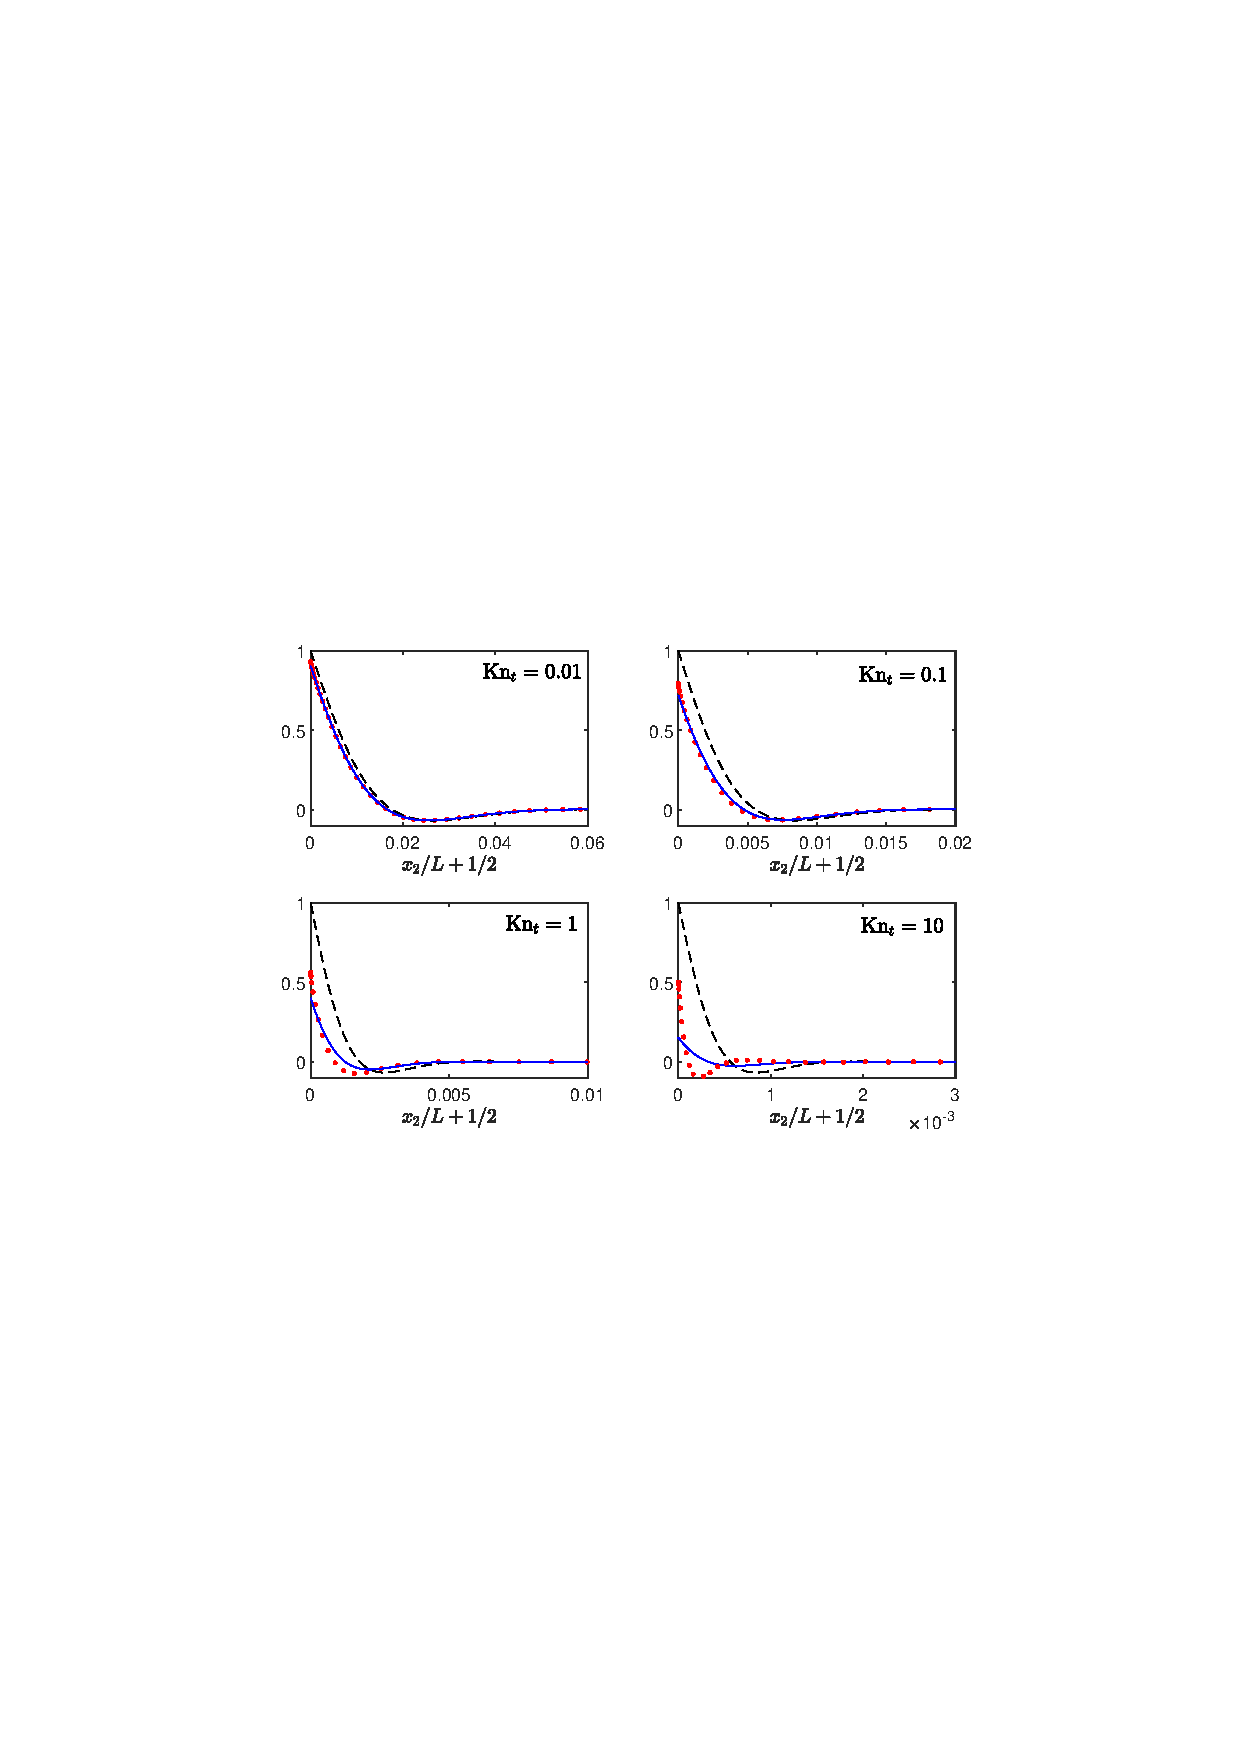
\includegraphics[width=0.8\columnwidth]{Introduction/IMG/Oscillatory_Couette_Route_NonEquilibrium.pdf}
	\caption{
		The real part of the flow velocity (normalized by the oscillation amplitude $u_w$) at $t=2m\pi/\varpi$ with $m=0,1,\cdots$, at different values of the temporal Knudsen number. The spatial Knudsen number is fixed at $\text{Kn}=0.001$. Dashed and solid lines are the solution of the NSF equation without and with the first-order velocity-slip boundary conditions~\cite{Sharipov2008Couette}, respectively, while circles are solutions from the linearized Boltzmann equation for HS gas, with the diffuse boundary condition. 
	}
	\label{Kn_t_region}
\end{figure}

Let us take the one-dimensional oscillatory Couette flow to demonstrate the rarefaction effects. The same setting as the planar Couette flow in the previous section is used, but now the plate at $x_2=-L/2$ oscillates in the $x_1$ direction with frequency $\varpi$ and amplitude $u_m$. Adopting the Navier-Stokes equations with the first-order velocity-slip boundary condition, the analytical solution for the gas velocity is obtained~\cite{Sharipov2008Couette}:
\begin{equation}\label{slip_solution_sharipov}
\begin{aligned}[b]
u_1=&u_w\exp(i\varpi{t})\frac{\sin\left[ (1+i)\delta_{rp}\sqrt{\text{Kn}_t}\left(\frac{1}{2}-\frac{x_2}{L}\right) \right]}{\sin\left[ (1+i)\delta_{rp}\sqrt{\text{Kn}_t} \right]}\\
&\times
\frac{1+(1+i)\sigma_P\sqrt{\text{Kn}_t}\cot\left[ (1+i)\delta_{rp}\sqrt{\text{Kn}_t} \left(\frac{1}{2}-\frac{x_2}{L}\right)\right]}
{1-2i\sigma_P^2{\text{Kn}_t}+2(1+i)\sigma_P\sqrt{\text{Kn}_t}\cot\left[ (1+i)\delta_{rp}\sqrt{\text{Kn}_t} \right]},
\end{aligned}
\end{equation}
where $i$ is the imaginary unit and $\sigma_P$ is the viscous slip coefficient. 
Here we take $\sigma_P=1$; more sophisticated calculations will be given in Chapter~\ref{chap:velocity_slip}. 
\index{viscous slip coefficient}



By comparing the numerical solution of the Boltzmann equation with the analytical solution, we are able to classify the flow regime based on the temporal Knudsen number. To isolate the rarefaction effects associated with the spatial Knudsen number, we set $\text{Kn}=0.001$. It is seen from Fig.~\ref{Kn_t_region} that, the slip solution~\eqref{slip_solution_sharipov} is valid up to $\text{Kn}_t\approx0.1$, while when $\text{Kn}_t=10$ the velocity profile from the Boltzmann equation is very close to the collisionless limit~\cite{Sharipov2008Couette}, indicating that the flow has entered the free-molecular regime. Therefore, we conclude that Fig.~\ref{Kn_region} ($\text{Kn}$ is replaced by $\text{Kn}_t$) can also be used to classify the four flow regimes in terms of the temporal Knudsen number, when the spatial Knudsen number is in the continuum flow regime. When both spatial and temporal Knudsen numbers are not small, stronger rarefaction effects are expected. 

%For example, Fig.~\ref{CouetteChapter1}  shows that, compared to $\text{Kn}=0.001$,  the curve of  $\text{Kn}=0.1$ saturates to the free-molecular limit faster.  

% so that the NSF equations break down at smaller values of Knudsen number,

%the Rayleigh-Brillouin scattering in Chapters~\ref{RBS:macroscopic} and~\ref{chap:fluctuation} is a good example in this regard.



\section{Molecular dynamics simulations}\label{MD_formula}
\index{molecular dynamics simulation}

Alternative methods should be adopted to study the RGD due to the breakdown of NSF equations in extreme conditions. Physically, when the intermolecular potential \index{intermolecular potential} $\phi$ is known, the molecular dynamics (MD) simulations, which is based on Newton's second law of motion, can be adopted to trace the movement of individual molecules:
\begin{equation}\label{Newtwon_equation}
m\frac{d^2\bm{x}_i}{dt^2}=\sum_j\bm{F}_{ij}, 
\quad \text{with~~} \bm{F}_{ij}=-\nabla\phi({r}_{ij}),
\end{equation}
where $\bm{x}_i$ is the position of the $i$-th molecule, $\nabla$ is the gradient operator, and ${r}_{ij}$ is the distance between the $i$-th and $j$-th molecules. 

When the position and velocity of individual molecule are known, macroscopic quantities can be obtained through ensemble average. Suppose there are $N$ molecules inside a volume $V$, the flow velocity $\bm{u}$ and temperature $T$ are given by:
\begin{eqnarray}
\bm{u}= \frac{1}{N} \sum_{i=1}^N \bm{v}_i,\\
T= \frac{m}{3Nk_B} \sum_{i=1}^N c^2.
\end{eqnarray}
where
\begin{equation}
	\bm{c}=\bm{v}-\bm{u}
\end{equation} 
is the peculiar velocity \index{peculiar velocity} and its magnitude is denoted by $c$. 
Independent runs for transient flows or time averaging for steady flows are needed to reduce the intrinsic noise in particle-based simulations.


\index{transport coefficient}
\index{translational thermal conductivity}

Transport coefficients such as the viscosity and heat conductivity that appear in the NSF equations can also be calculated in MD simulations, via the Green-Kubo formulas~\cite{Green1954,Kubo1957Japan}: \index{Green-Kubo}
\begin{eqnarray}
\mu=\frac{1}{V}\frac{1}{k_BT}\int_0^\infty 
\left\langle J_{xy}^p(0)J_{xy}^p(\tau)  \right\rangle d\tau, \\
\frac{4}{3}\mu+\mu_b=\frac{1}{V}\frac{1}{k_BT}\int_0^\infty 
\left\langle J_{xx}^p(0)J_{xx}^p(\tau)  \right\rangle d\tau,\\
\kappa=\frac{1}{V}\frac{1}{k_BT^2}\int_0^\infty 
\left\langle J_{x}^q(0)J_{x}^q(\tau)  \right\rangle d\tau, \label{GK_thermal}
\end{eqnarray}
where the brackets $\left\langle \cdots \right\rangle$ denote the canonical ensemble average, $\bm{J}^p= m\bm{c}_i\bm{c}_i-pV\bm{I}$ and $\bm{J}^q={E_i}\bm{c}_i$, with $\bm{I}$ being the identity matrix. For monatomic gas, $E_i=mc^2_i/2$ and $\kappa$ is the translational thermal conductivity $\kappa_{tr}$. For molecular gas, suppose $E_i=\epsilon_i$ is the internal energy of the $i$-th molecule, then Eq.~\eqref{GK_thermal} calculates the internal thermal conductivity $\kappa_i$; together with the translational thermal conductivity they form the total thermal conductivity $\kappa$.

\index{bulk viscosity}
\index{shear viscosity}
\index{thermal conductivity}
\index{translational thermal conductivity}
\index{internal thermal conductivity}


The MD simulation is also an indispensable tool to investigate the gas-surface interaction, which, together with the gas-gas interaction, determines the gas dynamics in wall-bounded problems. However, since it is limited to small spatial and temporal scales, the MD simulation cannot be used efficiently in rarefied gas flow simulations. Therefore, the gas kinetic theory, a mesoscopic theory that bridges the physics at the microscopic level and flow dynamics (phenomenon) at the macroscopic level, is needed.  


%\leir{extraction of critical parameters in molecular gas to feed into the kinetic models for simulation of rarefied gas flow }



